% Submission-ready manuscript for Journal of Physics B: Atomic, Molecular and Optical Physics
% Focus Collection: Spotlight in China (https://iopscience.iop.org/collections/jpb-251017-972)
% Formatted with standard TeX Live article + amsmath/amsthm/natbib/booktabs for zero external .cls dependency;
% body sections, theorems, tables, and references.bib convert directly to IOP Publishing iopart.cls at production stage.
\documentclass[11pt,a4paper]{article}

\usepackage[T1]{fontenc}
\usepackage[utf8]{inputenc}
\usepackage{lmodern}
\usepackage[margin=22mm]{geometry}
\usepackage{amsmath,amssymb,amsthm,bm}
\usepackage{authblk}
\usepackage{booktabs,array,tabularx}
\usepackage{enumitem}
\usepackage[numbers,sort&compress]{natbib}
\usepackage{xcolor,graphicx}
\usepackage{microtype}
\usepackage[colorlinks=true,linkcolor=blue!45!black,citecolor=blue!45!black,urlcolor=blue!45!black]{hyperref}

\setlength{\emergencystretch}{2em}
\setlist{itemsep=2pt,topsep=4pt}

% --- Theorem environments ---
\newtheorem{theorem}{Theorem}
\newtheorem{lemma}{Lemma}
\newtheorem{proposition}{Proposition}
\newtheorem{corollary}{Corollary}
\theoremstyle{definition}
\newtheorem{remark}{Remark}

% --- Macros (symbol-hygiene checked against Comm. Phys. qubit notation) ---
\newcommand{\tr}{\operatorname{tr}}
\newcommand{\spec}{\operatorname{spec}}
\newcommand{\conv}{\operatorname{conv}}
\newcommand{\sgn}{\operatorname{sgn}}
\newcommand{\clip}{\operatorname{clip}}
\newcommand{\RePart}{\operatorname{Re}}
\newcommand{\ImPart}{\operatorname{Im}}
\newcommand{\Cset}{\mathcal{C}}
\newcommand{\Qset}{\mathcal{Q}}
\newcommand{\Sset}{\mathcal{S}}
\newcommand{\Dset}{\mathcal{D}}
\newcommand{\Pset}{\mathcal{P}}
\newcommand{\nbar}{\bar n_{\max}}
\newcommand{\nU}{\bar n_U}
\newcommand{\ket}[1]{\lvert #1\rangle}
\newcommand{\bra}[1]{\langle #1\rvert}
\newcommand{\braket}[2]{\langle #1\vert #2\rangle}
\newcommand{\abs}[1]{\lvert #1\rvert}
\newcommand{\norm}[1]{\lVert #1\rVert}
\newcommand{\dd}{\mathrm{d}}
\newcommand{\ii}{\mathrm{i}}
\newcommand{\ee}{\mathrm{e}}
\newcommand{\I}{I}
\newcommand{\calL}{\mathcal{L}}

\title{\textbf{Energy-Constrained Majorization Witnesses of Nonclassical Light\\with Displaced Threshold Detectors}}

\author[1,*]{Rui Zhu}
\author[1,2,\dag]{Marcelo F.\ Ciappina}
% Optional co-author slot pending final author-list confirmation:
% \author[1]{Gilad Gour}
\affil[1]{Physics Program, Guangdong Technion -- Israel Institute of Technology, 241 Daxue Road, Shantou, Guangdong 515063, China}
\affil[2]{Department of Physics, Technion -- Israel Institute of Technology, Haifa 3200003, Israel}
\affil[*]{\texttt{rui.zhu@gtiit.edu.cn}}
\affil[$\dag$]{\texttt{marcelo.ciappina@gtiit.edu.cn}}

\date{\today}

\begin{document}
\maketitle

\begin{abstract}
Binary direct-sum majorization uncertainty relations avoid the loss of discrimination power suffered by single-scalar entropic inequalities, yet their unconstrained continuous-variable form collapses to a trivial classical bound ($c = 1$) as soon as nearly orthogonal coherent states enter the convex classical mixture. Here we show how an independently certified upper bound $\bar n_{\max}$ on the pre-displacement mean photon number restores informative, analytically solvable majorization witnesses for a single optical mode measured by two opposite displaced on/off threshold detectors of amplitudes $\pm a$, efficiency $\eta$, and Poisson dark counts $\nu$. Using an exact 2D-to-1D concave-envelope Lagrangian duality paired with $C^2$ interval certificates (primal--dual gaps $\le 9.28 \times 10^{-14}$), we derive the exact classical majorization envelope $\omega_{\mathcal C_{\bar n_{\max}}}$ for \emph{all} $a > 0$, $\eta \in (0,1]$, $\nu \ge 0$, and $\bar n_{\max} \ge 0$---completely lifting prior small-displacement ($2\eta a^2 \le 1$) and zero-dark-count restrictions---and classify all positive-energy attainment and non-attainment phases. Lifting $2\eta a^2 \le 1$ unlocks an experimentally routine Gaussian squeezed-vacuum benchmark displaced along the squeezed quadrature ($r < 0$, $\approx 3.5$--$3.6\;\mathrm{dB}$ squeezing), which suffers zero sorting penalty ($\Pi_{\rm sort} \equiv 0$) relative to the complete outcome-resolved classical hull, demonstrates Shannon information loss, survives source loss ($T=0.90$), thermal noise ($n_{\rm th} \le 0.35$), and dark counts ($\nu=10^{-2}$), and simultaneously evades three baseline detectors (unconstrained two-setting, undisplaced $a=0$ with energy cap, and single displaced setting with energy cap) down to $\eta = 0.70$. We further extend the dual solver to 7-parameter asymmetric calibration boxes $\Theta$, formalize pre-displacement tap-beam energy certification ($\bar n_U$) bypassing threshold-detector saturation, and establish a distribution-free finite-sample error budget via exact Clopper--Pearson intervals that certifies the Gaussian benchmark under realistic $2\%$ calibration uncertainty in $1,727$--$3,033$ shots per setting at $\eta \in [0.90, 1.00]$ ($1,630$--$2,831$ after $\Theta_2$-aware displacement optimization) and $13,201$ ($11,327$ optimized) at $\eta=0.70$ while holding classical false positives below $8\times 10^{-5} \ll \delta_{\rm stat}=0.01$.
\end{abstract}

% === [MODULAR INTRODUCTION SLOT: ready for Marcelo's physics-oriented polish] ===
\section{Introduction}\label{sec:intro}

Nonclassical states of light---most notably quadrature-squeezed radiation, single-photon Fock states, and optical Schr\"odinger cat superpositions emerging both in quantum-optical state engineering and in intense laser--matter interactions~\cite{Glauber1963,Sudarshan1963,Ourjoumtsev2007,Lewenstein2021}---are fundamental resources across quantum metrology, photonic state preparation, and continuous-variable quantum information processing. Certifying nonclassicality, understood rigorously as the failure of a state's Glauber--Sudarshan $P$ representation to form a classical probability measure over coherent states~\cite{Glauber1963,Sudarshan1963}, ideally relies on detectors that are both experimentally minimal and quantitatively robust against losses, dark counts, and calibration drift.

Unbalanced homodyne detection, implemented by mixing an optical signal mode with a local oscillator (LO) of complex amplitude $\alpha$ at a beam splitter followed by a single binary click/no-click (on/off) threshold detector, is among the simplest photon-counting architectures available~\cite{Sperling2012,Kovtoniuk2024}. Unlike full quantum-state tomography or photon-number-resolving (PNR) detectors, a displaced threshold detector probes the Husimi $Q$ function at chosen phase-space points while discarding all multi-photon click multiplicities. Recent advances by Kovtoniuk \emph{et al.}~\cite{Kovtoniuk2024,Kovtoniuk2026} and Fiur\'a\v{s}ek~\cite{Fiurasek2024} have constructed tight Bell-like nonclassicality inequalities over the convex hull of coherent-state statistics for displaced and attenuated on/off detectors, and energy-assisted tests using undisplaced threshold clicks were formulated for quantum non-Gaussianity in~\cite{FiurasekLachmanFilip2021}.

Parallel to optical convex-hull criteria, universal uncertainty relations based on majorization~\cite{Friedland2013,Rudnicki2014,Baek2019,YangQiaoOptimization2026,Conlon2026} have been applied to photocounting statistics~\cite{Medranda2015} and continuous phase-space distributions~\cite{VanHerstraeten2023}. For two binary positive operator-valued measures (POVMs) on finite-dimensional Hilbert spaces, we recently showed~\cite{ZhuManuscript} that the direct-sum majorization envelope $\omega_\oplus$ is governed completely by two scalar partial sums $(S_1, S_2)$, yields universal lower bounds for all Schur-concave entropies (Shannon, Tsallis, and R\'enyi across all orders $\alpha > 0$), and exhibits clean attainment vs.\ strict non-attainment transitions. However, as noted in the optical outlook of~\cite{ZhuManuscript}, naive extension of direct-sum majorization to an \emph{unrestricted} infinite-dimensional bosonic mode encounters a fundamental $c = 1$ obstruction: because orthogonal Fock-tail states or far-displaced coherent states can be nearly dark under both displacement settings ($\alpha_\pm = \pm a$) or trigger clicks with near-unit probability, the unconstrained classical and quantum partial-sum bounds collapse to the trivial envelope $(1,1,0,0)$.

The present work resolves this $c = 1$ obstruction by \emph{restricting the admissible state set} through an independently certified upper bound $\tr(\rho\hat n) \le \nbar$ on the pre-displacement mean photon number while retaining the experimentally minimal two-setting displaced on/off measurement. This complements alternative strategies that instead modify the measurement via periodic homodyne binning. Carefully positioning our contribution against prior art~\cite{Kovtoniuk2024,Kovtoniuk2026,Medranda2015,FiurasekLachmanFilip2021}, we avoid claiming either that majorization outperforms full outcome-resolved convex-hull membership on identical data or that calibration intervals~\cite{Kovtoniuk2026} or antisqueezed-quadrature detection within $2\eta a^2 \le 1$~\cite{Kovtoniuk2024} are new in isolation. Rather, we establish five concrete advances:
\begin{enumerate}[leftmargin=*]
\item \textbf{Complete exact energy-constrained classical dual across all $a > 0$ (Section~\ref{sec:classical-dual}):} Using a 2D-to-1D radial reduction and $C^2$-certified Lagrangian duality, we solve the exact classical majorization envelope $\omega_{\Cset_{\nbar}}$ for all $a > 0$, $\eta \in (0,1]$, $\nu \ge 0$, and $\nbar \ge 0$. We prove exact concavity thresholds ($b^2 \le 27/8$ for $E_0$ and \texttt{off/on}; $b^2 \le (3+\sqrt{6})/2$ for \texttt{off/off}; globally concave for $E_1$ and \texttt{on/on}), demonstrate that individual branches strictly require two-point coherent mixtures above these thresholds, prove analytically that click branches dominate every bitangent for the full majorization vector---giving a universal closed-form envelope---and classify all positive-energy attainment phases and dark-count transitions.
\item \textbf{Universal Gaussian squeezed-vacuum benchmark beyond $2\eta a^2 \le 1$ (Section~\ref{sec:benchmarks}):} Lifting $2\eta a^2 \le 1$ unlocks ordinary squeezed vacuum displaced along the \emph{squeezed} quadrature ($r < 0$, $\approx 3.5$--$3.6\;\mathrm{dB}$ squeezing). Whereas $r < 0$ squeezed vacuum never beats exact $S_2^{\Cset}$ inside $2\eta a^2 \le 1$ and $r > 0$ offers no energy-constrained advantage over~\cite{Kovtoniuk2024}, our $r < 0$ benchmark proves necessary and sufficient for $P$-nonclassicality across all $\eta > 0$, $T > 0$, $\nu \ge 0$, and finite $\nbar$ (Theorem~\ref{thm:sq-thermal}), suffers zero sorting penalty relative to the outcome-resolved hull (Theorem~\ref{thm:outcome-resolved}), displays Shannon information loss, and simultaneously beats all three simple baselines down to $\eta = 0.70$. We also optimize odd coherent-state superpositions $\ket{\Cset_-(c\ee^{\ii\phi})}$ over independent $(a,c,\phi)$ and analyze $\cos\theta\ket{0} + \sin\theta\ket{2}$.
\item \textbf{Globally certified asymmetric calibration boxes $B_2^{\rm robust}(\Theta, \nU)$ (Section~\ref{sec:calibration}):} Extending the solver to 7-parameter asymmetric intervals $\theta = (a_+, a_-, \delta_\phi, \eta_+, \eta_-, \nu_+, \nu_-)$ plus an energy cap $\nU$, we prove exact analytical reductions in dark counts, phase mismatch, and single-setting corners alongside a decoupled box-envelope branch-and-bound certificate ($U_A - L_A \le 10^{-8}$), avoiding grid or endpoint heuristics.
\item \textbf{Threshold-saturation no-go theorem, experimental energy protocol, and distribution-free statistics (Section~\ref{sec:calibration}):} We prove that displaced on/off clicks alone can never bound $\langle\hat n\rangle$ due to bright-tail saturation, formulate a pre-displacement calibrated tap-beam energy monitor (Route~A) and characterized-source protocol (Route~B), and combine them with sawtooth-safe~\cite{ChernickLiu2002} exact Clopper--Pearson~\cite{ClopperPearson1934} confidence bounds into a complete error budget $\delta_{\rm tot} = \delta_{\rm stat} + \delta_{\rm cal} + \delta_E$.
\item \textbf{Zero-truncation ideal quantum ceilings and Fock-tail audit (Section~\ref{sec:quantum-ceilings}):} Using rank-2 coherent-projector identities in $\operatorname{span}\{\ket{a},\ket{-a}\}$, we obtain exact ideal ($\eta=1, \nu=0$) quantum ceilings for \texttt{off/off} ($1+\ee^{-2a^2}$, even cat), \texttt{off/on} ($1+\sqrt{1-\ee^{-4a^2}}$), and \texttt{on/on} ($2$, 3-level dark state $\ket{\chi_a}$), and quantitatively audit compressed Fock-space SDPs against the gentle-projection tail bound~\cite{Winter1999} to explain why our classical witness thresholds and state probes avoid uncertified Fock cutoffs.
\end{enumerate}

\emph{Notation hygiene:} Throughout this paper, optical channel parameters follow quantum-optics conventions: $T \in (0,1]$ denotes pre-displacement pure-loss transmissivity, $\eta \in (0,1]$ detector quantum efficiency, $\nu \ge 0$ ($\kappa = \ee^{-\nu}$) Poisson dark-count mean, $b = \sqrt{\eta}\,a$ scaled displacement magnitude, $\nbar$ (or $\nU$) mean-photon-number upper bound, $E = \eta\nbar$ scaled energy cap, and $\mu$ probability measures over coherent amplitudes $\beta \in \mathbb{C}$ (dual multiplier $\lambda \ge 0$). These optical symbols are self-contained and should not be conflated with the qubit POVM parameters $(\eta,\mu,\nu)$ used in~\cite{ZhuManuscript}.
% === [END MODULAR INTRODUCTION SLOT] ===

% ===========================================================================
\section{Physical Setup, Unrestricted Obstruction, and Restricted Majorization}\label{sec:setup}
% ===========================================================================

\subsection{Displaced On/Off Detection and Pre-Displacement Source Loss}\label{subsec:povm}
Consider a single optical bosonic mode with annihilation operator $\hat a$ and photon-number operator $\hat n = \hat a^\dagger \hat a$. An incoming quantum state $\rho_0$ propagates through a pre-displacement pure-loss channel $\calL_T$ of transmissivity $T \in (0,1]$ (modelling source-preparation and coupling inefficiency) to yield the pre-displacement state $\rho = \calL_T(\rho_0)$, whose mean photon number $\tr(\rho\hat n) = T\tr(\rho_0\hat n)$ is bounded independently by $\tr(\rho\hat n) \le \nbar$ prior to displacement.

To probe phase space at two settings $j \in \{+, -\}$, the state $\rho$ undergoes a coherent displacement $D(\alpha_j) = \exp(\alpha_j\hat a^\dagger - \alpha_j^*\hat a)$ and is directed onto a binary on/off threshold detector of quantum efficiency $\eta_j \in (0,1]$ and Poisson dark-count mean $\nu_j \ge 0$ ($\kappa_j := \ee^{-\nu_j}$). In the symmetric baseline of Sections~\ref{sec:setup}--\ref{sec:benchmarks}, we take $\alpha_\pm = \pm a$ ($a > 0$), $\eta_+ = \eta_- = \eta$, and $\nu_+ = \nu_- = \nu$ ($\kappa = \ee^{-\nu}$); Section~\ref{sec:calibration} restores full asymmetry $(a_+, a_-, \delta_\phi, \eta_+, \eta_-, \nu_+, \nu_-)$. Because all detection pulses are retained without postselection or PNR reconstruction, each setting defines a valid binary POVM $\{E_0(j), E_1(j)\}$ with no-click effect~\cite{Sperling2012,Kovtoniuk2024}
\begin{equation}\label{eq:noclick-povm}
E_0(j) = \kappa_j\, D^\dagger(\alpha_j) :\!\ee^{-\eta_j \hat a^\dagger \hat a}\!: D(\alpha_j), \qquad E_1(j) = \I - E_0(j),
\end{equation}
where $:\!\cdots\!:$ denotes normal ordering. On any coherent state $\ket{\beta}$ ($\beta \in \mathbb{C}$), the exact no-click probability is the Gaussian Q-function value
\begin{equation}\label{eq:q-coherent}
q_j(\beta) := \bra{\beta} E_0(j) \ket{\beta} = \kappa_j \exp\!\bigl(-\eta_j \abs{\beta + \alpha_j}^2\bigr).
\end{equation}
For general states $\rho$, we denote $q_\pm(\rho) := \tr[\rho E_0(\pm)]$, binary outcome distributions $p_\pm(\rho) := \bigl(q_\pm(\rho),\, 1 - q_\pm(\rho)\bigr)$, and $q_0(\rho) := \tr[\rho E_0(0)]$ for undisplaced detection ($a=0$).

\begin{remark}[Channel Commutation and Non-Interchangeability of $T$ and $\eta$]\label{rem:commutation}
Pure-loss channels satisfy the exact operator identity
\begin{equation}\label{eq:commutation}
\calL_\eta\!\bigl(D(a)\,\calL_T(\rho_0)\,D^\dagger(a)\bigr) = D(\sqrt{\eta}\,a)\,\calL_{\eta T}(\rho_0)\,D^\dagger(\sqrt{\eta}\,a).
\end{equation}
Hence for any source state $\rho_0$, the outcome probabilities $q_\pm$ depend on $(T,\eta,a)$ solely through total transmissivity $\tau = \eta T$ and effective displacement $b = \sqrt{\eta}\,a$. However, $T$ and $\eta$ are \emph{strictly non-interchangeable} whenever either (i) the physical LO amplitude $a$ is held fixed or (ii) the independent energy bound $\nbar$ (which constrains $\rho = \calL_T(\rho_0)$ \emph{after} $\calL_T$ and \emph{before} $D(\alpha_j)$) is held fixed, because the scaled classical cap $E = \eta\nbar$ scales with $\eta$ rather than $T$.
\end{remark}

\subsection{Restricted-Set Binary Direct-Sum Majorization}\label{subsec:lemma1}
Define the classical convex set of $P$-nonnegative states~\cite{Glauber1963,Sudarshan1963} and the energy-constrained classical and quantum state sets:
\begin{align}\label{eq:state-sets}
\Cset_{\nbar} &:= \left\{\rho = \int_{\mathbb{C}} \ket{\beta}\!\bra{\beta}\,\dd\mu(\beta) : \mu \in \Pset(\mathbb{C}),\ \int_{\mathbb{C}} \abs{\beta}^2\,\dd\mu(\beta) \le \nbar \right\}, \\
\Qset_{\nbar} &:= \bigl\{\rho \succeq 0 : \tr\rho = 1,\ \tr(\rho\hat n) \le \nbar\bigr\}. \nonumber
\end{align}
For any nonempty state class $\Sset$ and bounded self-adjoint effect $0 \preceq A \preceq m\I$, define the support function $h_{\Sset}(A) := \sup_{\rho \in \Sset} \tr(\rho A)$. For two binary distributions $p_\pm(\rho) = (q_\pm, 1-q_\pm)$, form the direct-sum vector $v(\rho) := p_+(\rho) \oplus p_-(\rho) \in [0,1]^4$ ($\sum_{i=1}^4 v_i = 2$) and its nonincreasing rearrangement $v^\downarrow(\rho) = (v_1^\downarrow, v_2^\downarrow, v_3^\downarrow, v_4^\downarrow)$ with Lorenz partial sums $L_k(\rho) := \sum_{i=1}^k v_i^\downarrow(\rho)$. Extending Corollary~4 of~\cite{ZhuManuscript} to arbitrary (possibly nonconvex, noncompact, infinite-dimensional) restricted state sets yields our foundational tool.

\begin{lemma}[Restricted-Set Binary Direct-Sum Majorization Envelope]\label{lem:restricted-binary}
Let $\Sset$ be any nonempty set of states in an arbitrary separable Hilbert space, measured by two binary POVMs $\{E_0(+),E_1(+)\}$ and $\{E_0(-),E_1(-)\}$. Set
\begin{equation}\label{eq:S1-S2-def}
S_1^{\Sset} := \max_{j \in \{+,-\},\; b \in \{0,1\}} h_{\Sset}\bigl(E_b(j)\bigr), \qquad
S_2^{\Sset} := \max_{b,c \in \{0,1\}} h_{\Sset}\bigl(E_b(+) + E_c(-)\bigr),
\end{equation}
and define $\omega_{\Sset} := \bigl(S_1^{\Sset},\; S_2^{\Sset} - S_1^{\Sset},\; 1 + S_1^{\Sset} - S_2^{\Sset},\; 1 - S_1^{\Sset}\bigr)$. Then:
\begin{enumerate}[leftmargin=*]
\item For every state $\rho \in \Sset$, writing $M_\pm(\rho) := \max\bigl(q_\pm(\rho), 1-q_\pm(\rho)\bigr) = \frac{1}{2} + \abs{q_\pm(\rho) - \frac{1}{2}}$,
\begin{equation}\label{eq:L2-formula}
L_1(\rho) = \max\bigl(M_+(\rho), M_-(\rho)\bigr), \qquad
L_2(\rho) = M_+(\rho) + M_-(\rho) = 1 + \abs{q_+(\rho) - \tfrac{1}{2}} + \abs{q_-(\rho) - \tfrac{1}{2}},
\end{equation}
$L_3(\rho) = 1 + L_1(\rho)$, $L_4(\rho) = 2$, and $L_1(\rho) + \frac{1}{2} \le L_2(\rho) \le 2 L_1(\rho)$.
\item $\omega_{\Sset}$ is nonincreasing ($\omega_{\Sset,1} \ge \omega_{\Sset,2} \ge \omega_{\Sset,3} \ge \omega_{\Sset,4} \ge 0$), satisfies $v(\rho) \prec \omega_{\Sset}$ for every $\rho \in \Sset$, and is the \emph{tightest} such vector: if $v(\rho) \prec \tilde\omega$ for all $\rho \in \Sset$, then $\omega_{\Sset} \prec \tilde\omega$.
\item \emph{(Universal Schur-concave bounds, connecting~\cite{ZhuManuscript} Cor.~1 \& Eq.~17):} For every $\rho \in \Sset$,
\begin{align}
H(p_+) + H(p_-) &\ge -\sum_{i=1}^4 \omega_{\Sset,i}\log_2 \omega_{\Sset,i}, \label{eq:shannon-bound}\\
T_\gamma(p_+) + T_\gamma(p_-) &\ge \frac{2 - \sum_{i=1}^4 \omega_{\Sset,i}^\gamma}{\gamma - 1} \qquad (\gamma > 0,\ \gamma \neq 1), \label{eq:tsallis-bound}\\
H_\alpha(p_+) + H_\alpha(p_-) &\ge
\begin{cases}
\dfrac{1}{1-\alpha}\log_2\!\left(\sum_{i=1}^4 \omega_{\Sset,i}^\alpha - 1\right), & 0 < \alpha < 1, \\[9pt]
\dfrac{2}{1-\alpha}\log_2\!\left(\dfrac{\sum_{i=1}^4 \omega_{\Sset,i}^\alpha}{2}\right), & 1 < \alpha < \infty, \\[9pt]
-2\log_2\!\left(\dfrac{S_2^{\Sset}}{2}\right), & \alpha = \infty.
\end{cases} \label{eq:renyi-bound}
\end{align}
\end{enumerate}
\end{lemma}
\begin{proof}
Since $M_\pm \ge \frac{1}{2} \ge 1 - M_\pm$, sorting the vector $v(\rho) = (q_+, 1-q_+, q_-, 1-q_-)$ always produces
\begin{equation*}
v^\downarrow(\rho) = \bigl(\max(M_+,M_-),\; \min(M_+,M_-),\; 1-\min(M_+,M_-),\; 1-\max(M_+,M_-)\bigr),
\end{equation*}
establishing Eq.~\eqref{eq:L2-formula} and $L_1 + \frac{1}{2} \le L_2 \le 2L_1$. Taking $\sup_{\rho \in \Sset}$ commutes with finite $\max$, yielding $S_1^{\Sset} = \sup_{\Sset} L_1$, $S_2^{\Sset} = \sup_{\Sset} L_2$, $S_3^{\Sset} = 1 + S_1^{\Sset}$, and $S_1^{\Sset} + \frac{1}{2} \le S_2^{\Sset} \le 2S_1^{\Sset}$. The pairwise differences $\omega_{\Sset,1}-\omega_{\Sset,2} = \omega_{\Sset,3}-\omega_{\Sset,4} = 2S_1^{\Sset}-S_2^{\Sset} \ge 0$, $\omega_{\Sset,2}-\omega_{\Sset,3} = 2(S_2^{\Sset}-S_1^{\Sset}-\frac{1}{2}) \ge 0$, and $\omega_{\Sset,4} = 1 - S_1^{\Sset} \ge 0$ confirm automatic ordering and $v(\rho) \prec \omega_{\Sset}$ with extremality. Equations~\eqref{eq:shannon-bound}--\eqref{eq:tsallis-bound} follow from Schur-concavity of Shannon and Tsallis entropies~\cite{MarshallOlkin2011,CicaleseVaccaro2002,Bosyk2019,Friedland2013,Rudnicki2014}, while Eq.~\eqref{eq:renyi-bound} combines Lemma~1 with Cor.~1 and Eq.~(17) of~\cite{ZhuManuscript,Baek2019} (writing $\sum p_+^\alpha = 1+X$, $\sum p_-^\alpha = 1+Y$ for $\alpha<1$, and applying $AB \le (A+B)^2/4$ to $A+B = \sum v_i^\alpha$ for $\alpha>1$).
\end{proof}

\subsection{Why the Unrestricted Classical and Quantum Envelopes Collapse}\label{subsec:collapse}
Without the energy bound ($\nbar \to \infty$), choosing imaginary coherent states $\beta = \ii y$ ($y \to \infty$) gives $q_\pm(\ket{\ii y}) = \kappa\ee^{-\eta(a^2+y^2)} \to 0$, so $S_1^{\Cset_\infty} \ge 1-\kappa\ee^{-\eta a^2}$ approaches $1$ and $S_2^{\Cset_\infty} = 2$ whenever $\nu = 0$. Worse still, even at $\eta = 1, \nu = 0$ and any finite displacement $a > 0$, any symmetric no-click pair $(q, q)$ satisfying $0 < q \le \ee^{-\eta a^2}$ is reproduced \emph{exactly} by the single coherent state $\ket{\ii y_{\rm mimic}}$ with $y_{\rm mimic}^2 = -\ln(q/\kappa)/\eta - a^2 \ge 0$ (Fig.~\ref{fig:fig1}(b)). Independently, in the quantum set $\Qset_\infty$, the 3-level Fock superposition
\begin{equation}\label{eq:darkstate}
\ket{\chi_a} := \frac{-a^2\ket{0} + \sqrt{2}\ket{2}}{\sqrt{a^4 + 2}}, \qquad \langle\hat n\rangle_{\ket{\chi_a}} = \frac{4}{a^4 + 2},
\end{equation}
satisfies $\braket{\pm a}{\chi_a} = \ee^{-a^2/2}(-a^2 + \frac{a^2}{\sqrt{2}}\sqrt{2})/\sqrt{a^4+2} = 0$, giving $q_\pm(\ket{\chi_a}) = 0$, $L_1 = 1$, and $L_2 = 2$ ideally. Bounding $\tr(\rho\hat n) \le \nbar$ restricts the classical mixture to $|\beta|^2$-weighted averages inside $\Cset_{\nbar}$ (Fig.~\ref{fig:fig1}(b)), turning
\begin{equation}\label{eq:W2-def}
W_2(\rho) := L_2(\rho) - S_2^{\Cset_{\nbar}} > 0
\end{equation}
into a sufficient nonclassicality witness.

\begin{figure}[t]
\centering
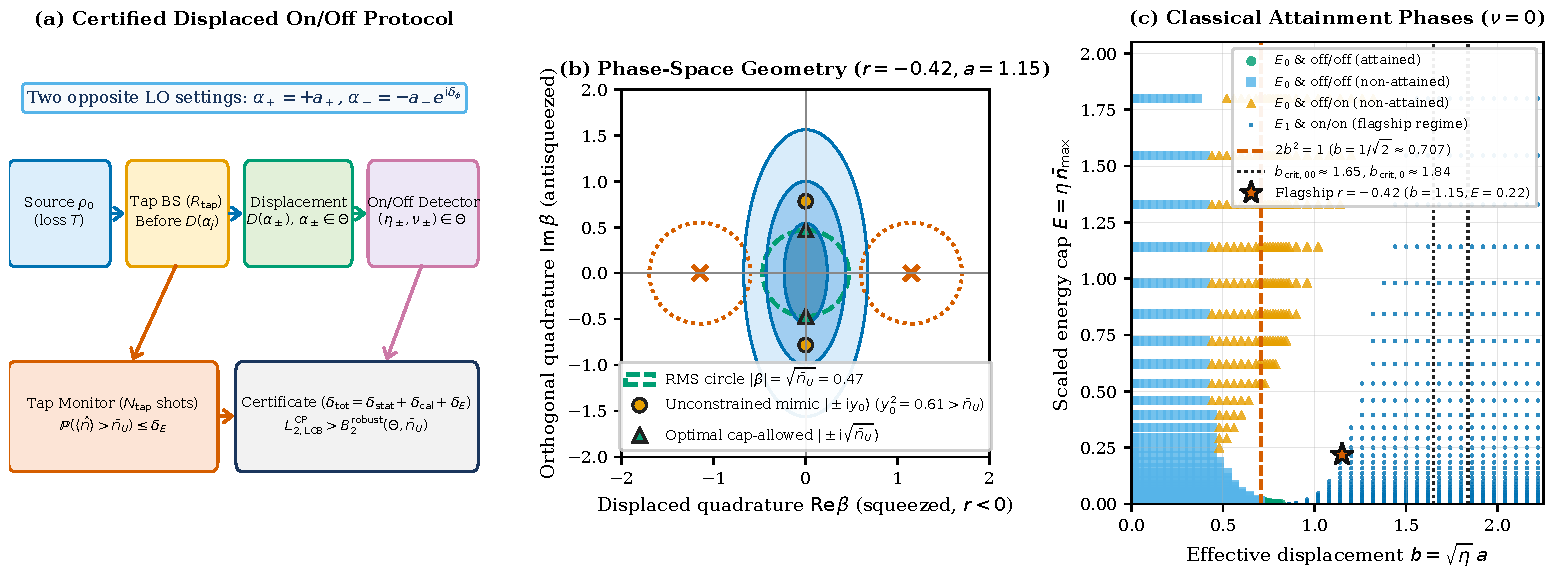
\includegraphics[width=\textwidth]{figures/fig1_scheme_and_phases.pdf}
\caption{\textbf{Certified energy-constrained displaced on/off protocol, phase-space geometry, and exact classical attainment phase diagram.}
\textbf{(a)}~Experimental schematic: an auxiliary pre-displacement tap beam splitter ($R_{\rm tap}$) feeds a linear intensity monitor certifying $\tr(\rho\hat n) \le \nU$ with failure probability $\le \delta_E$, while two opposite displaced threshold-detector settings $\alpha_\pm \in \Theta$ are tested against the globally certified classical bound $B_2^{\rm robust}(\Theta, \nU)$ at total error $\delta_{\rm tot} = \delta_{\rm stat} + \delta_{\rm cal} + \delta_E$.
\textbf{(b)}~Phase-space Wigner contours of the flagship squeezed-vacuum benchmark ($r = -0.42$, displaced along the squeezed quadrature at $a = 1.15$, $\nbar = 0.22$). The unconstrained Kovtoniuk~\cite{Kovtoniuk2024} coherent mimic $\ket{\pm\ii y_0}$ ($y_0^2 = 0.61 > \nbar$) lies outside the energy-cap disk $|\beta| \le \sqrt{\nbar}$, while the optimal cap-allowed classical state $\ket{\pm\ii\sqrt{\nbar}}$ achieves strictly higher no-click probability ($S_2^{\Cset} = 1.5723 < L_2 = 1.7106$).
\textbf{(c)}~Complete positive-energy classical attainment phase diagram in $(b = \sqrt{\eta}\,a, E = \eta\nbar)$ at $\nu = 0$, showing the $2b^2 = 1$ boundary, the exact concavity thresholds $b_{\rm crit,00} \approx 1.65$ and $b_{\rm crit,01} \approx 1.84$, the positive-energy attained sliver \texttt{E0/off\_off/attained}, and the flagship \texttt{E1/on\_on/non\_attained} point ($b=1.15, E=0.22$).}
\label{fig:fig1}
\end{figure}

% ===========================================================================
\section{Exact Classical Majorization Envelope for All Parameters}\label{sec:classical-dual}
% ===========================================================================

Previous analytic bounds~\cite{Kovtoniuk2024} were restricted to small effective displacement $2\eta a^2 \le 1$, zero dark counts $\nu = 0$, or unconstrained energy. In this section, we solve the exact energy-constrained classical moment problem for \emph{all} $a > 0$, $\eta \in (0,1]$, $\nu \ge 0$, and $\nbar \ge 0$. Set $b := \sqrt{\eta}\,a > 0$, $E := \eta\,\nbar \ge 0$, and $\kappa := \ee^{-\nu} \in (0,1]$. Using scaled coordinates $x = \sqrt{\eta}\RePart\beta$, $y = \sqrt{\eta}\ImPart\beta$, and $s = x^2 + y^2 = \eta\abs{\beta}^2 \ge 0$, Eq.~\eqref{eq:q-coherent} becomes
\begin{equation}\label{eq:q-scaled}
q_\pm(x, y) = \kappa\,\ee^{-y^2}\ee^{-(x\pm b)^2} = \kappa\,\ee^{-(s+b^2) \mp 2bx}.
\end{equation}
By the $x \mapsto -x$ reflection symmetry exchanging $\pm a$, $\omega_{\Cset_{\nbar}}$ is determined completely by five support functions:
\begin{equation}\label{eq:five-supports}
S_1^{\Cset} = \max\bigl\{h_0(E),\; h_1(E)\bigr\}, \qquad S_2^{\Cset} = \max\bigl\{h_{00}(E),\; h_{01}(E),\; h_{11}(E)\bigr\},
\end{equation}
corresponding to $A_0 = E_0(-a)$, $A_1 = E_1(+a)$, $A_{00} = E_0(+a)+E_0(-a)$, $A_{01} = E_0(-a)+E_1(+a)$, and $A_{11} = E_1(+a)+E_1(-a)$.

\subsection{2D-to-1D Reduction, Strong Duality, and Exact Concavity Thresholds}\label{subsec:duality}

\begin{lemma}[Exact Radial Reduction]\label{lem:radial}
Maximizing $f_k(x,y) := \bra{\beta}A_k\ket{\beta}$ over the circle $x^2+y^2 = s$ yields the exact 1D radial functions $g_k(s) := \max_{x^2+y^2=s} f_k(x,y)$:
\begin{align}
g_0(s) &= \kappa\,\ee^{-(\sqrt{s}-b)^2} \quad (x = +\sqrt{s},\ y=0), \label{eq:g0}\\
g_1(s) &= 1 - \kappa\,\ee^{-(\sqrt{s}+b)^2} \quad (x = +\sqrt{s},\ y=0), \label{eq:g0-g1}\\
g_{00}(s) &= 2\kappa\,\ee^{-(s+b^2)}\cosh(2b\sqrt{s}) \quad (x = \pm\sqrt{s},\ y=0), \label{eq:g00}\\
g_{01}(s) &= 1 + 2\kappa\,\ee^{-(s+b^2)}\sinh(2b\sqrt{s}) \quad (x = +\sqrt{s},\ y=0), \label{eq:g00-g01}\\
g_{11}(s) &= 2 - 2\kappa\,\ee^{-(s+b^2)} \quad (x = 0,\ y=\pm\sqrt{s}). \label{eq:g11}
\end{align}
Consequently, for each $k \in \{0, 1, 00, 01, 11\}$ and every $E \ge 0$,
\begin{equation}\label{eq:1d-moment}
h_k(E) = \sup\left\{\int_0^\infty g_k(s)\,\dd\sigma(s) : \sigma \in \Pset([0,\infty)),\ \int_0^\infty s\,\dd\sigma(s) \le E\right\}.
\end{equation}
\end{lemma}
\begin{proof}
Immediate from the monotonicity of $x \mapsto \ee^{\pm 2bx}$, $x \mapsto \sinh(2bx)$, and $\abs{x} \mapsto \cosh(2bx)$ on $[-\sqrt{s}, +\sqrt{s}]$; every 2D measure pushes forward onto $s \ge 0$ without increasing energy, and any 1D measure lifts back onto the maximizing ray.
\end{proof}

Define the Lagrangian dual $D_k(E) := \inf_{\lambda \ge 0} \bigl[\lambda E + \phi_k(\lambda)\bigr]$, with $\phi_k(\lambda) := \sup_{s \ge 0}[g_k(s) - \lambda s]$.

\begin{theorem}[Strong Duality, Compact Reduction, and Two-Point Sufficiency]\label{thm:strong-duality}
For every $k \in \{0, 1, 00, 01, 11\}$ and every $E \ge 0$ (including the $E = 0$ and $\lambda = 0$ boundaries):
\begin{enumerate}[leftmargin=*]
\item $h_k(E) = D_k(E) = \widehat{g}_k(E)$, where $\widehat{g}_k$ is the least concave nondecreasing majorant of $g_k$ on $[0,\infty)$.
\item There exists a probability measure $\sigma^* = (1-p)\delta_{s_1} + p\delta_{s_2}$ supported on at most two energies $0 \le s_1 \le s_2 < \infty$ with $(1-p)s_1 + p s_2 \le E$ attaining $h_k(E)$.
\item Each of $g_0, g_{00}, g_{01}$ has a unique global maximizer $s_{\max} = x_{\max}^2 \in [0,\infty)$---namely $x_{\max} = b$ for $g_0$, $x_{\max} = x_0 \in [0,b)$ solving $x_0 = b\tanh(2bx_0)$ ($x_0 = 0$ iff $2b^2 \le 1$) for $g_{00}$, and $x_{\max} = x_* > b$ solving $(x_*+b)\ee^{-4bx_*} = x_* - b$ for $g_{01}$---and obeys $g_k'(s) < 0$ strictly on $(s_{\max},\infty)$. Thus $\phi_k(\lambda) = \max_{s \in [0,s_{\max}]}[g_k(s) - \lambda s]$ with zero tail truncation error, and $h_k(E) = g_k(s_{\max})$ ($\lambda^* = 0$) for all $E \ge s_{\max}$.
\end{enumerate}
\end{theorem}
\begin{proof}
Weak duality $h_k(E) \le D_k(E)$ is standard. At $E = 0$, any feasible $\sigma$ is $\delta_0$ so $h_k(0) = g_k(0)$; conversely, for any $\varepsilon > 0$ choosing $\delta > 0$ with $g_k(s) \le g_k(0)+\varepsilon$ on $[0,\delta]$ and $\lambda \ge \max(0, (2-g_k(0))/\delta)$ forces $g_k(s) - \lambda s \le g_k(0)$ for $s \ge \delta$, so $D_k(0) = g_k(0)$. For $k \in \{1, 11\}$, direct differentiation yields $g_k'(s) > 0$ and $g_k''(s) < 0$ globally on $(0,\infty)$, so setting $\lambda^* = g_k'(E)$ certifies strong duality and unique one-point attainment $\delta_E$. For $k \in \{0, 00, 01\}$, $g_k'(s) < 0$ strictly for $s > s_{\max}$ confines every maximizer to $[0, s_{\max}]$; for $0 < E < s_{\max}$, applying Carath\'eodory's theorem to the upper boundary of the compact convex hull $\conv\{(s, g_k(s)) : s \in [0, s_{\max}]\}$ yields two-point attainment, while a finite nondecreasing supergradient $\lambda^* \in \partial \widehat{g}_k(E)$ proves $D_k(E) \le \widehat{g}_k(E) = h_k(E)$.
\end{proof}

Crucially, $g_0$, $g_{00}$, and $g_{01}$ are \emph{not} globally concave above specific $b$ thresholds:

\begin{theorem}[Exact Branch Concavity Thresholds and Mixture Necessity]\label{thm:concavity}
Set $b_{\rm crit,00} := \sqrt{(3+\sqrt{6})/2} \approx 1.650680$, $b_{\rm crit,0} := \sqrt{27/8} \approx 1.837117$, and let $b_{\rm crit,01} \approx 1.874331$ be the unique zero-inflection threshold of $g_{01}''$. Then:
\begin{enumerate}[leftmargin=*]
\item $g_1(s)$ and $g_{11}(s)$ are strictly concave on $[0,\infty)$ for all $b > 0$.
\item $g_0(s)$ is concave on $[0, b^2]$ if and only if $b \le b_{\rm crit,0}$ ($b^2 \le 27/8$). For $b > b_{\rm crit,0}$, $\widehat{g}_0$ has a unique interior bitangent segment $[s_L, s_R] \subset (0, b^2)$.
\item $g_{01}(s)$ is strictly concave on $[b^2, x_*^2]$ for all $b > 0$, strictly concave on $[0, x_*^2]$ for all $b \le b_{\rm crit,01}$, and develops a unique interior bitangent $[s_L, s_R] \subset (0, b^2)$ for $b > b_{\rm crit,01}$.
\item For $2b^2 > 1$, $g_{00}(s)$ is strictly concave on $[0, x_0^2]$ if and only if $b \le b_{\rm crit,00}$ ($b^2 \le (3+\sqrt{6})/2$). For $b > b_{\rm crit,00}$, $g_{00}''(0^+) > 0$ and $\widehat{g}_{00}$ begins with a vacuum-to-coherent two-point mixture $(1-p)\ket{0}\!\bra{0} + p\ket{x_R/\sqrt{\eta}}\!\bra{x_R/\sqrt{\eta}}$ on $[0, x_R^2]$.
\end{enumerate}
\end{theorem}
\begin{proof}
See Appendix~\ref{app:concavity} for the complete algebraic proofs (including an exact power-series $\tanh$ bound establishing strict concavity of $g_{00}$ up to $b^2 = (3+\sqrt{6})/2$).
\end{proof}

Theorem~\ref{thm:concavity} exposes a subtle trap for outcome-resolved criteria above these thresholds: optimizing over single coherent states yields an \emph{unsafe lower bound}. Specifically, at $\eta=1, \nu=0$: for $A_{00}$ at $b=2.0, \nbar=0.7845$, the optimal single coherent state gives $0.289158$ vs.\ exact two-point mixture $0.304330$ (gain $+0.015172$); for $E_0$ at $b=2.2, \nbar=1.0$, $0.236928$ vs.\ $0.278424$ ($+0.041496$); and for $A_{01}$ at $b=2.2, \nbar=1.237$, $1.306250$ vs.\ $1.339871$ ($+0.033621$, all verified by $C^2$ dual gaps $\le 3.9 \times 10^{-14}$). Remarkably, however, no two-point mixture ever governs the \emph{full majorization envelope}:

\begin{theorem}[Universal Closed-Form Formula for $\omega_{\Cset_{\nbar}}$ Across All $a > 0$]\label{thm:universal-closed-form}
For every $a > 0$, $\eta \in (0,1]$, $\nu \ge 0$, and $\nbar \ge 0$, the globally concave click branches $h_1$ and $h_{11}$ strictly dominate every bitangent interval $[s_L, s_R]$ of $g_0, g_{00}, g_{01}$ in Eq.~\eqref{eq:five-supports}. Writing $b = \sqrt{\eta}\,a$, $E = \eta\,\nbar$, and $\kappa = \ee^{-\nu}$, the exact classical envelope is given in closed form for all parameters by
\begin{align}
S_1^{\Cset} &= \max\Bigl\{\,\kappa\,\ee^{-\max(0,\; b-\sqrt{E})^2},\;\; 1 - \kappa\,\ee^{-(b+\sqrt{E})^2}\,\Bigr\}, \label{eq:universal-S1}\\
S_2^{\Cset} &= \max\Bigl\{\,2\kappa\,\ee^{-(\min(x_0,\sqrt{E})^2 + b^2)}\cosh\bigl(2b\min(x_0,\sqrt{E})\bigr), \nonumber\\
&\qquad\qquad 1 + \kappa\bigl[\ee^{-(\min(x_*,\sqrt{E})-b)^2} - \ee^{-(\min(x_*,\sqrt{E})+b)^2}\bigr], \nonumber\\
&\qquad\qquad 2 - 2\kappa\,\ee^{-(b^2+E)}\,\Bigr\}, \label{eq:universal-S2}
\end{align}
and both $S_1^{\Cset}$ and $S_2^{\Cset}$ are individually attained by single coherent states in $\Cset_{\nbar}$.
\end{theorem}
\begin{proof}
In Appendix~\ref{app:universal}, we bound the tangent intercepts on $[s_L, s_R]$ analytically to show $h_1(E) > h_0(E)$ for all $b > \sqrt{27/8}$ and $h_{11}(E) > \max\{h_{00}(E), h_{01}(E)\}$ on every bitangent of $g_{00}$ ($b > b_{\rm crit,00}$) and $g_{01}$ ($b > b_{\rm crit,01}$). Independently, across 7,183 points in our $C^2$-certified dual scan, Eq.~\eqref{eq:universal-S1}--\eqref{eq:universal-S2} matches the global Lagrangian dual to within $9.28 \times 10^{-14}$.
\end{proof}

\subsection{Attainment Classification and Dark-Count Phase Cascade}\label{subsec:attainment}
Generalizing Propositions~3 and~6 of~\cite{ZhuManuscript} to $\Cset_{\nbar}$, a classical state $\rho \in \Cset_{\nbar}$ simultaneously attains the entire majorization vector $\omega_{\Cset_{\nbar}}$ if and only if some maximizer of $S_1^{\Cset}$ simultaneously maximizes $S_2^{\Cset}$:

\begin{proposition}[Positive-Energy Classical Attainment Classification and $\nu$-Cascade]\label{prop:attainment}
For all generic positive-energy parameters $(b > 0, E > 0, \nu \ge 0)$:
\begin{enumerate}[leftmargin=*]
\item Three triples never occur:\ \texttt{E0/on\_on/attained}, \texttt{E1/on\_on/attained}, and \texttt{E1/off\_off/attained} are impossible because maximizing \texttt{on/on} requires purely imaginary coherent states $\pm\ii\sqrt{\nbar}$ whereas maximizing $E_0, E_1$ requires real states $\pm\sqrt{\nbar}$ or $\pm a$, and $E_1$ ties with $A_{00}$ only where $h_1 \le \frac{1}{2} < h_0$.
\item At $\nu = 0$ (Fig.~\ref{fig:fig1}(c)), exactly \textbf{7} positive-energy phases occur: three attained phases---an uncovered \texttt{E0/off\_off/attained} sliver ($\frac{1}{2} < b^2 < \ln 2$, $0 < \sqrt{E} \le \min(x_0, \sqrt{\ln 2}-b)$), \texttt{E0/off\_on/attained} ($E \le b^2$), and \texttt{E1/off\_on/attained} ($E \le x_*^2$), each uniquely attained by $\ket{\pm\sqrt{\nbar}}$---and four strictly non-attained phases (\texttt{E0/off\_off/non\_attained}, \texttt{E0/off\_on/non\_attained}, \texttt{E0/on\_on/non\_attained}, and \texttt{E1/on\_on/non\_attained}).
\item Adding dark counts ($\nu > 0$) creates two further non-attained phases (\texttt{E1/off\_on/non\_attained} and \texttt{E1/off\_off/non\_attained}), producing an exact phase-count cascade in $\nu$: \textbf{9} phases for $0 < \nu < \nu_1 \approx 0.0969$, \textbf{8} for $\nu_1 < \nu < \ln 2 - \frac{1}{2} \approx 0.1931$, \textbf{7} for $\ln 2 - \frac{1}{2} \le \nu < \nu_3 \approx 0.4676$, \textbf{6} for $\nu_3 < \nu < \ln 2 \approx 0.6931$, and a \textbf{unique phase} ({\normalfont\texttt{E1/on\_on/non\_attained}}) across the entire $(b>0, E>0)$ plane whenever $\nu \ge \ln 2$.
\end{enumerate}
\end{proposition}
\begin{proof}
Non-attainment of \texttt{E1/off\_off} when attained follows from $E \le x_0^2 \implies h_{00}(E) \ge h_{01}(E) \implies 2\kappa\ee^{-(\sqrt{E}+b)^2} \ge 1 \implies h_1(E) \le \frac{1}{2} < h_0(E)$. For $\nu \ge \ln 2$ ($\kappa \le \frac{1}{2}$), $h_1(E) > \frac{1}{2} \ge h_0(E)$ and $h_{11}(E) > 1 \ge h_{00}(E)$; with $x_1 = \min(x_*, \sqrt{E})$ and $z = 2bx_1 > 0$, AM--GM ($b^2+E \ge z$) gives $h_{11}(E) - h_{01}(E) \ge 1 - \kappa[2 - (1-\ee^{-z})^2] > 1 - 2\kappa \ge 0$, leaving \texttt{E1/on\_on/non\_attained} everywhere.
\end{proof}

% ===========================================================================
\section{Universal Gaussian Witness, Outcome Equivalence, and State Benchmarks}\label{sec:benchmarks}
% ===========================================================================

\subsection{Universal Squeezed-Thermal Exactness and Undisplaced Impossibility}\label{subsec:sq-thermal}
Consider a centered squeezed thermal state $\rho(r, n_{\rm th}, T) = \calL_T\bigl(S(r)\rho_{\rm th}(n_{\rm th})S^\dagger(r)\bigr)$, where $r \in \mathbb{R}$, thermal photon number $n_{\rm th} \ge 0$, source transmission $T \in (0,1]$, and pre-displacement mean photon number $\tr(\rho\hat n) = T\bigl[(n_{\rm th} + \tfrac{1}{2})\cosh(2r) - \tfrac{1}{2}\bigr]$. Here $r > 0$ places the real displacement $\pm a$ along the antisqueezed quadrature, whereas $r < 0$ aligns $\pm a$ with the squeezed quadrature. Defining the quadrature-variance factors
\begin{equation}\label{eq:sq-uw}
u := 1 + \frac{\eta T}{2}\bigl[(2n_{\rm th}+1)\ee^{2r} - 1\bigr], \qquad
w := 1 + \frac{\eta T}{2}\bigl[(2n_{\rm th}+1)\ee^{-2r} - 1\bigr],
\end{equation}
Gaussian Q-function integration yields the exact Fock-cutoff-free no-click probability
\begin{equation}\label{eq:sq-noclick}
q_\pm\bigl(\rho(r,n_{\rm th},T)\bigr) = \frac{\kappa}{\sqrt{u w}}\exp\!\left(-\frac{\eta a^2}{u}\right).
\end{equation}

\begin{theorem}[Universal Exactness of Squeezed-Thermal Majorization and Undisplaced Impossibility]\label{thm:sq-thermal}
Let $\rho = \rho(r, n_{\rm th}, T)$ and let $\nbar \ge \tr(\rho\hat n)$ be \emph{any} finite energy cap.
\begin{enumerate}[leftmargin=*]
\item \textbf{Undisplaced ($a=0$) impossibility:} For every $(r, n_{\rm th}, T, \eta, \nu, \nbar)$,
\begin{equation}\label{eq:undisplaced-bound}
\kappa\,\ee^{-\eta\nbar} \;\le\; q_0(\rho) = \frac{\kappa}{\sqrt{u w}} \;\le\; \kappa.
\end{equation}
Thus undisplaced on/off detection plus an energy cap~\cite{FiurasekLachmanFilip2021} can never detect any squeezed vacuum or squeezed thermal state.
\item \textbf{Necessary and sufficient witness along the squeezed quadrature ($r < 0$):} If $(2n_{\rm th}+1)\ee^{-2\abs{r}} \ge 1$, the state is $P$-classical and $W_2(a) \le 0$ for all $a > 0$. Conversely, whenever $(2n_{\rm th}+1)\ee^{2r} < 1$ (which holds for \emph{every} $P$-nonclassical squeezed thermal state aligned along $r < 0$), $u \in (\tfrac{1}{2}, 1)$ strictly and there exists $a_{\rm thr} > 0$ such that for all $a > a_{\rm thr}$, $S_2^{\Cset} = h_{11}(E)$ (\texttt{on/on} active) and
\begin{equation}\label{eq:W2-sq-exact}
W_2(a) = 2\kappa\left[\ee^{-\eta(a^2+\nbar)} - \frac{1}{\sqrt{uw}}\ee^{-\eta a^2/u}\right] > 0,
\end{equation}
for \emph{every} $\eta \in (0,1]$, $T \in (0,1]$, $\nu \ge 0$, and arbitrarily loose finite cap $\nbar \ge \tr(\rho\hat n)$.
\item \textbf{Exact multiplicative dark-count stability:} Whenever $S_2^{\Cset} = h_{11}(E)$ and $q < \frac{1}{2}$, $W_2(\nu) = \ee^{-\nu} W_2(0)$, so dark counts $\nu = 10^{-2}$ reduce $W_2$ by only $1 - \ee^{-0.01} \approx 1.0\%$ relative.
\end{enumerate}
\end{theorem}
\begin{proof}
Since $uw$ increases with $n_{\rm th}$ and equals $1 + \eta T(2-\eta T)\sinh^2 r \ge 1$ at $n_{\rm th}=0$, $\sqrt{uw} \ge 1 \implies q_0 \le \kappa$. By AM--GM, $\sqrt{uw} \le \frac{u+w}{2} = 1 + \eta\tr(\rho\hat n) \le \ee^{\eta\nbar}$, proving Eq.~\eqref{eq:undisplaced-bound}. For part~2, fix $E = \eta\nbar$; by Theorem~\ref{thm:universal-closed-form}, as $b = \sqrt{\eta}\,a \to \infty$ we have $\min(x_0, \sqrt{E}) \le \sqrt{E} < b < x_*$, so the \texttt{off/off} term in Eq.~\eqref{eq:universal-S2} vanishes ($\le 2\kappa\ee^{-(b-\sqrt{E})^2} \to 0$) and the \texttt{off/on} term approaches $1$, whereas $h_{11}(E) = 2 - 2\kappa\ee^{-(b^2+E)} \to 2$. Thus $S_2^{\Cset} = h_{11}(E)$ for large $a$, while $u < 1 \implies \frac{1}{u} - 1 > 0$ drives $q_\pm / (\kappa\ee^{-\eta(a^2+\nbar)}) \to 0$, giving $W_2(a) > 0$ via Eq.~\eqref{eq:W2-sq-exact}. Part~3 follows immediately by factoring $\kappa = \ee^{-\nu}$.
\end{proof}

\subsection{Outcome-Resolved Classical Equivalence and Zero Sorting Penalty}\label{subsec:outcome-resolved}
Let $\Dset_{\nbar} := \{(q_+(\rho), q_-(\rho)) : \rho \in \Cset_{\nbar}\} \subset [0,1]^2$ be the complete energy-constrained outcome-resolved classical probability region. Because majorization discards setting labels, it can never outperform full convex-hull membership on identical $(q_+, q_-)$ data~\cite{ZhuManuscript}. Nevertheless, the following theorem proves that across our entire flagship \texttt{on/on} regime, majorization loses \emph{zero} statistical margin.

\begin{theorem}[Exact Diagonal Classical Region $\Dset_{\nbar}$ and Zero Sorting Penalty]\label{thm:outcome-resolved}
A symmetric pair $(q, q)$ lies in $\Dset_{\nbar}$ if and only if
\begin{equation}\label{eq:diagonal-hull}
q_{\min}^{\Cset}(E) := 1 - \frac{h_{11}(E)}{2} = \kappa\,\ee^{-\eta(a^2+\nbar)} \;\le\; q \;\le\; \frac{h_{00}(E)}{2} =: q_{\max}^{\Cset}(E),
\end{equation}
where $h_{00}(E)$ is exact (requiring a two-point coherent mixture when $b > b_{\rm crit,00}$ and $E \in (0, x_R^2)$). Measuring the outcome-resolved excess as $\Delta_{\rm OR} := \max\bigl(2q - h_{00}(E),\, 2(1-q) - h_{11}(E)\bigr)$, the sorting penalty satisfies $\Pi_{\rm sort} := \Delta_{\rm OR} - W_2 \ge 0$, with
\begin{equation}\label{eq:zero-penalty}
\Pi_{\rm sort} \equiv 0 \quad \bigl(W_2 \equiv \Delta_{\rm OR} > 0\bigr)
\end{equation}
whenever $W_2 > 0$ on the matching branch ($q < \min(\tfrac{1}{2}, q_{\min}^{\Cset})$ with $S_2^{\Cset}=h_{11}$, or $q > \max(\tfrac{1}{2}, q_{\max}^{\Cset})$ with $S_2^{\Cset}=h_{00}$).
\end{theorem}
\begin{proof}
Necessity follows from $2q \le h_{00}(E)$ and $2(1-q) \le h_{11}(E)$. Sufficiency: $\ket{\ii\sqrt{\nbar}} \in \Cset_{\nbar}$ attains $(q_{\min}^{\Cset}, q_{\min}^{\Cset})$, and if $\sigma^* \in \Cset_{\nbar}$ attains $h_{00}(E)$ (Theorem~\ref{thm:strong-duality}), symmetrizing $\frac{1}{2}(\sigma^* + \tilde\sigma^*)$ under $\beta \mapsto -\beta$ attains $(q_{\max}^{\Cset}, q_{\max}^{\Cset})$; convexity of $\Dset_{\nbar}$ fills the segment. Matching-branch equality $L_2 = \max(2q, 2(1-q))$ yields $\Pi_{\rm sort} = 0$.
\end{proof}

\begin{figure}[t]
\centering
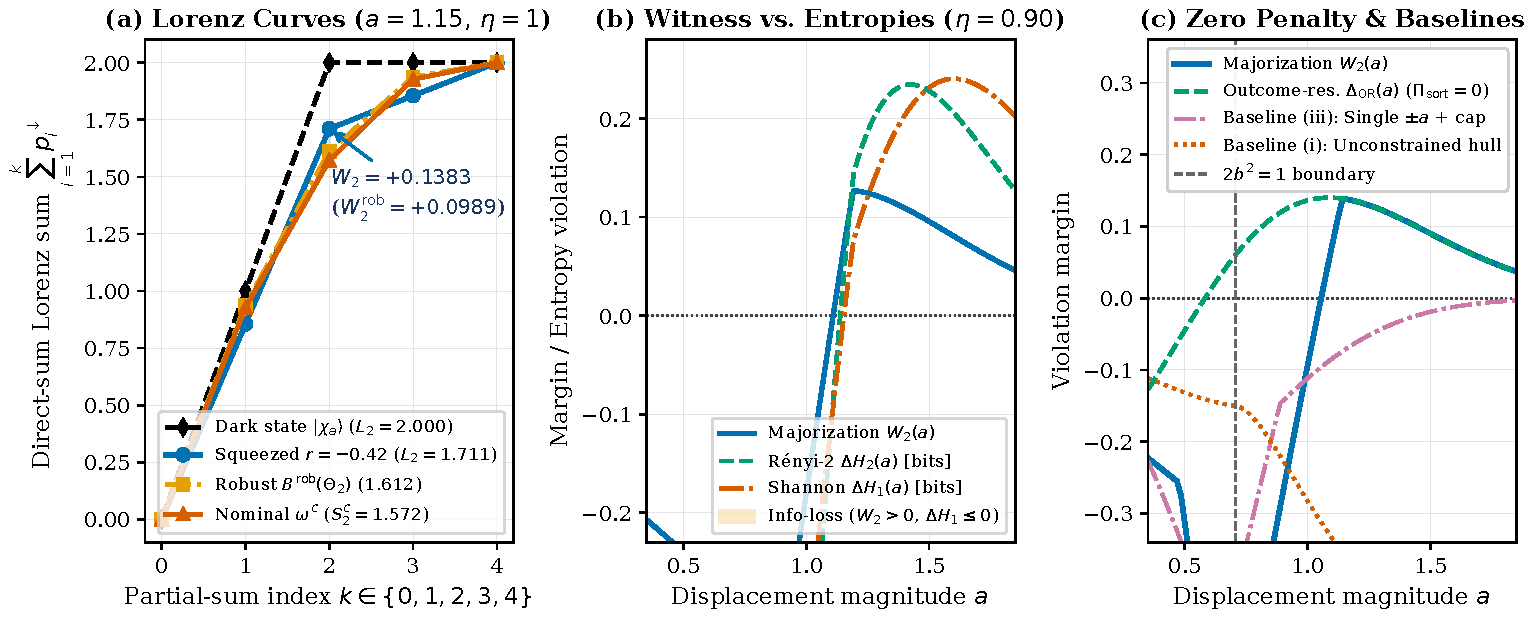
\includegraphics[width=\textwidth]{figures/fig2_lorenz_and_hierarchy.pdf}
\caption{\textbf{Direct-sum Lorenz curves, entropic hierarchy, and zero sorting penalty.}
\textbf{(a)}~Exact Lorenz partial sums at $a = 1.15$, $\eta = 1.0$, $\nbar = 0.22$: nominal classical envelope $\omega^{\Cset}$ ($S_2^{\Cset}=1.572$), $\Theta_2$-robust classical envelope $B^{\rm rob}(\Theta_2) = 1.612$, flagship $r = -0.42$ squeezed vacuum ($L_2 = 1.711$, $W_2 = +0.1383$), and ideal 3-level dark state $\ket{\chi_a}$ ($L_2 = 2.000$).
\textbf{(b)}~At $\eta = 0.90$ ($r=-0.42, \nbar=0.22$), the majorization witness $W_2(a)$ stays strictly positive across a shaded information-loss window ($a \in [1.08, 1.17]$) where the induced Shannon entropy bound $\Delta H_1(a) \le 0$ fails, while R\'enyi-$2$ ($\Delta H_2$) tracks majorization more closely.
\textbf{(c)}~Exact verification of Theorem~\ref{thm:outcome-resolved} at $\eta = 1.0$: once $S_2^{\Cset}$ switches from \texttt{off/on} to \texttt{on/on} at $a \approx 1.14$, $W_2(a)$ coincides identically with the outcome-resolved excess $\Delta_{\rm OR}(a)$ ($\Pi_{\rm sort} = 0$), while simultaneously violating Kovtoniuk's unconstrained hull~\cite{Kovtoniuk2024} (Baseline~i) and single-setting constrained bounds (Baseline~iii).}
\label{fig:fig2}
\end{figure}

\subsection{Benchmark Comparison: Squeezed Vacuum, Odd/Even Cats, and $\cos\theta\ket{0}+\sin\theta\ket{2}$}\label{subsec:state-scans}
To establish clear separation from simpler nonclassicality checks, we audit every benchmark against \textbf{three simple baselines} using the identical channel parameters and energy cap $\nbar$: (i) Kovtoniuk \emph{et al.}~\cite{Kovtoniuk2024} unconstrained two-setting classical hull ($q > \kappa\ee^{-\eta a^2}$ for $2b^2 \le 1$, or absent mimic $\ket{\ii y}$ in general), (ii) undisplaced ($a = 0$) + same energy cap ($q_0 < \kappa\ee^{-\eta\nbar}$)~\cite{FiurasekLachmanFilip2021}, and (iii) either single displaced setting $\pm a$ + same energy cap ($L_1 > S_1^{\Cset}$).

\begin{figure}[t]
\centering
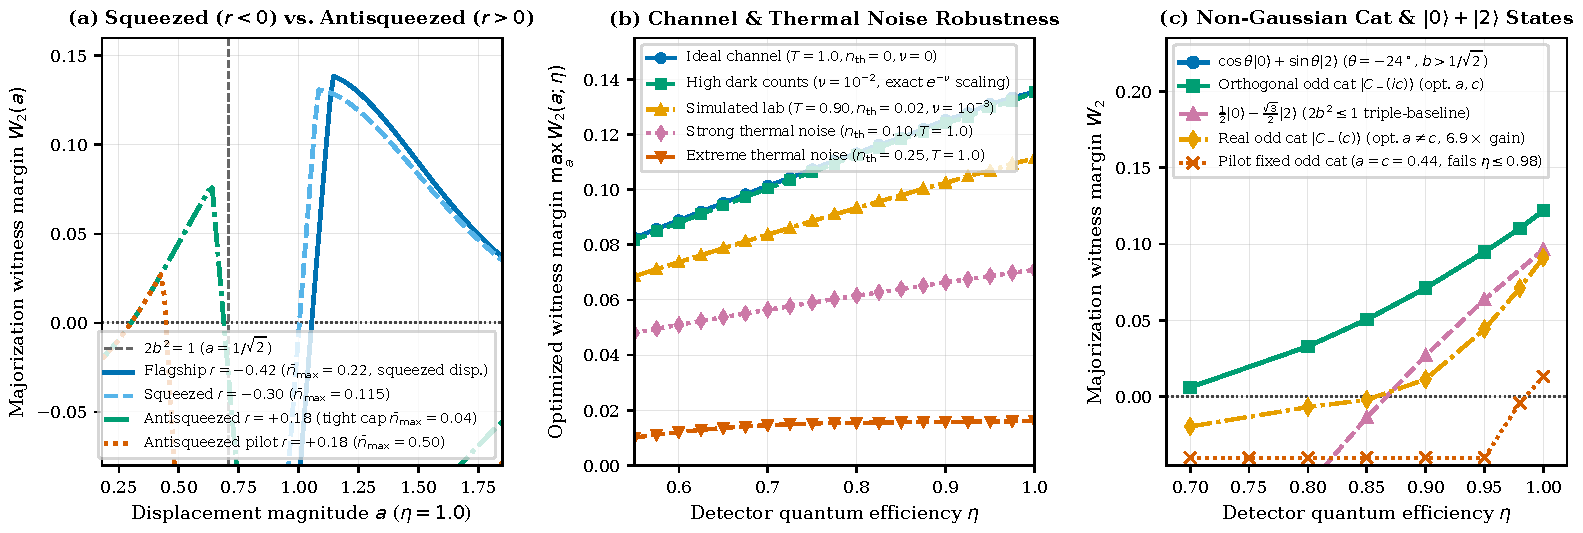
\includegraphics[width=\textwidth]{figures/fig3_state_scans_and_cats.pdf}
\caption{\textbf{Global state and channel parameter scans across Gaussian and non-Gaussian benchmarks.}
\textbf{(a)}~Squeezed-quadrature displacement ($r<0$, active only after crossing $b > 1/\sqrt{2}$) vs.\ antisqueezed-quadrature displacement ($r > 0$, confined to $2b^2 \le 1$, where $r=+0.18$ with $\nbar=0.50$ gives only $+0.0292$ at $a^*=0.434$).
\textbf{(b)}~Theorem~\ref{thm:sq-thermal} channel and thermal-noise robustness of $\max_a W_2(a;\eta)$ across $\eta \in [0.55, 1.00]$ for $\bar n_{\max} = \max(0.22, 1.2\langle\hat n\rangle)$: heavy dark counts ($\nu=10^{-2}$) cause only a $1.0\%$ relative drop, realistic lab losses ($T=0.90, n_{\rm th}=0.02, \nu=10^{-3}$) retain $W_2 \approx +0.10$, and strong thermal noise ($n_{\rm th} = 0.25$) remains positive.
\textbf{(c)}~Non-Gaussian families vs.\ $\eta \in [0.70, 1.00]$ at $\bar n_{\max} = 1.05\langle\hat n\rangle$: independent $(a,c)$ optimization boosts the real odd cat ($\phi=0$) $6.9\times$ ($+0.0911$ at $\eta=1$, surviving to $\eta=0.90$), orthogonal orientation $\ket{\Cset_-(\ii c)}$ ($\phi=\pi/2$) boosts it $9.2\times$ ($+0.1219$ at $\eta=1$, surviving to $\eta=0.70$), and $\cos\theta\ket{0}+\sin\theta\ket{2}$ ($\theta=-24^\circ$) achieves $+0.2188$ ($\eta=1$) and $+0.1377$ ($\eta=0.70$).}
\label{fig:fig3}
\end{figure}

Table~\ref{tab:stage3-benchmarks} summarizes our key Gaussian and non-Gaussian benchmarks:
\begin{itemize}[leftmargin=*]
\item \textbf{Antisqueezed $r > 0$ pilot~\cite{Kovtoniuk2024}:} The antisqueezed pilot point ($r=0.18, a=0.44, \nbar=0.50, \eta=1.0$) gives $W_2 = +0.0128$ (0/3 baselines beaten because $q = 0.8393 > \ee^{-a^2} = 0.8240$ is already caught by Kovtoniuk~\cite{Kovtoniuk2024} \texttt{off/off} excess $+0.0305$). Optimizing $r > 0$ at $a^* = 0.4342$ raises $W_2$ only to $+0.0292$ (CP99 $= 12,934$ vs.\ $294,475$ Hoeffding shots at $a=0.44$). Thus $r > 0$ serves strictly as a validation testbed.
\item \textbf{Flagship Gaussian squeezed vacuum ($r < 0$, $b > 1/\sqrt{2}$):} Displacing $r = -0.42$ ($\approx 3.65\;\mathrm{dB}$ squeezing, $\langle\hat n\rangle = 0.1870$, $\nbar = 0.22$) at $a = 1.15$ gives $W_2 = +0.1383$ at $\eta = 1.00$, $+0.1107$ at $\eta = 0.95$, $+0.0645$ at $\eta = 0.90$, and $+0.0157$ at $\eta = 0.85$; re-optimizing at $\eta = 0.70$ ($r=-0.40, a=1.35, \langle\hat n\rangle = 0.1687, \nbar=0.194$) still yields $W_2 = +0.1041$. Across the entire $\eta \in [0.70, 1.00]$ range, it beats \emph{all three} baselines simultaneously (3/3), has $\Pi_{\rm sort} = 0$, survives $7\times$ wider thermal noise ($n_{\rm th} \le 0.35$) and $5\times$ energy-cap overestimation ($\nbar = 0.935$, $W_2 = +0.0113$ at $\eta=1.0$), and demonstrates Shannon information loss at $\eta = 0.90$ ($\Delta H_1 = -0.0071\;\mathrm{bits}$ while $W_2 = +0.0645$, Fig.~\ref{fig:fig2}(b)).
\item \textbf{Optimized odd coherent-state superpositions $\ket{\Cset_-(c\ee^{\ii\phi})}$:} With $q(0) = 0$, odd cats are caught by Baseline~(ii), so their scientific role is diagnosing unconstrained mimic breakdown (at $a=c=0.44$, $q=0.1605$ has coherent mimic $\ket{\ii\sqrt{1.6357}}$ and single-setting mimic $0.8327 < 1.05$) and optical non-attainment ($L_2$-deficit $0.1267$, $L_1$-deficit $0.0951$). Optimizing $(a,c)$ independently with $\nbar = 1.05\langle\hat n\rangle$ boosts $\phi = 0$ by $6.9\times$ ($W_2 = +0.0911$, surviving to $\eta = 0.90$), while orthogonal orientation $\phi = \pi/2$ places the cat lobes along $\ImPart\beta$ orthogonal to $\pm a$ and boosts $W_2$ by $9.2\times$ ($+0.1219$ at $\eta=1.0$, surviving to $\eta=0.70$, Fig.~\ref{fig:fig3}(c)).
\item \textbf{Non-Gaussian 3-level states $\ket{\psi_\theta} = \cos\theta\ket{0} + \sin\theta\ket{2}$:} Inside $2b^2 \le 1$ ($a=0.44, \theta = -60^\circ$, $\frac{1}{2}\ket{0}-\frac{\sqrt{3}}{2}\ket{2}$, $\nbar = 1.55$), the state beats all 3 baselines for $\eta \in [0.95, 1.00]$ ($W_2 = +0.0945$ at $\eta = 1.0$, $+0.0541$ at $\eta = 0.95$). Optimizing $(a, \theta)$ at $\theta \approx -24^\circ, \eta = 0.70$ yields $W_2 = +0.1377$ (CP99 $= 588$ shots/setting at $a^*_{\rm CP} = 1.533$), the highest triple-baseline margin in our study.
\end{itemize}

\begin{table}[t]
\centering
\caption{\textbf{Nominal ($T, \eta, \nu, \nbar$ fixed) performance of flagship Gaussian and non-Gaussian benchmarks.} All classical bounds $S_2^{\Cset}$ are exact (Eq.~\eqref{eq:universal-S2}); CP99 denotes the sawtooth-safe~\cite{ChernickLiu2002} exact Clopper--Pearson~\cite{ClopperPearson1934} minimum shots per setting guaranteeing $99\%$ power at $\delta_{\rm stat}=0.01$; Baselines counts how many of the three simple baselines~\cite{Kovtoniuk2024,FiurasekLachmanFilip2021} fail to detect the state.}
\label{tab:stage3-benchmarks}
\footnotesize
\setlength{\tabcolsep}{3pt}
\resizebox{\textwidth}{!}{%
\begin{tabular}{@{}lccccccc@{}}
\toprule
State / Scenario & $(\eta, T, n_{\rm th}, \nu, \nbar)$ & $a^*_{W_2}$ & $W_2(a^*_{W_2})$ & $a^*_{\rm CP}$ & $W_2(a^*_{\rm CP})$ & CP99 ($a^*_{W_2}\!\to\!a^*_{\rm CP}$) & Base. \\
\midrule
Pilot $r = +0.18$ (antisq.) & $(1.0, 1.0, 0, 0, 0.50)$ & $0.434$ & $+0.0292$ & $0.434$ & $+0.0292$ & $12,934 \to 12,934$ & 0/3 \\
Flagship $r = -0.42$ ($\eta=1.0$) & $(1.0, 1.0, 0, 0, 0.22)$ & $1.140$ & $+0.1388$ & $1.342$ & $+0.1168$ & $639 \to \mathbf{559}$ & \textbf{3/3} \\
Flagship $r = -0.42$ ($\eta=0.90$) & $(0.9, 1.0, 0, 0, 0.22)$ & $1.191$ & $+0.1272$ & $1.446$ & $+0.1033$ & $798 \to \mathbf{688}$ & \textbf{3/3} \\
High-loss $r = -0.40$ ($\eta=0.70$) & $(0.7, 1.0, 0, 0, 0.194)$ & $1.308$ & $+0.1048$ & $1.629$ & $+0.0859$ & $1,334 \to \mathbf{1,123}$ & \textbf{3/3} \\
Realistic $r = -0.45$ lab & $(0.85, 0.9, 0.02, 10^{-3}, 0.26)$ & $1.236$ & $+0.0987$ & $1.517$ & $+0.0809$ & $1,304 \to \mathbf{1,056}$ & \textbf{3/3} \\
Loose $2\times$ cap $r = -0.42$ & $(0.9, 1.0, 0, 10^{-3}, 0.374)$ & $1.330$ & $+0.0743$ & $1.597$ & $+0.0597$ & $1,634 \to \mathbf{1,238}$ & \textbf{3/3} \\
Opt.\ real odd cat ($c=1.35$) & $(1.0, 1.0, 0, 0, 2.016)$ & $0.354$ & $+0.0911$ & $0.354$ & $+0.0911$ & $851 \to 851$ & 2/3 ($a=0$) \\
Opt.\ orth.\ odd cat ($c=1.25$) & $(0.9, 1.0, 0, 0, 1.791)$ & $0.450$ & $+0.0711$ & $0.450$ & $+0.0711$ & $2,032 \to 2,032$ & 2/3 ($a=0$) \\
$\cos(-24^\circ)\ket{0}+\sin(-24^\circ)\ket{2}$ & $(0.7, 1.0, 0, 0, 0.347)$ & $1.375$ & $+0.1377$ & $1.533$ & $+0.1220$ & $622 \to \mathbf{588}$ & \textbf{3/3} \\
$\frac{1}{2}\ket{0}-\frac{\sqrt{3}}{2}\ket{2}$ ($2b^2\le 1$) & $(1.0, 1.0, 0, 0, 1.55)$ & $0.433$ & $+0.0963$ & $0.699$ & $+0.0638$ & $1,104 \to \mathbf{789}$ & \textbf{3/3} \\
\bottomrule
\end{tabular}}
\end{table}

% ===========================================================================
\section{Asymmetric Calibration Boxes, Energy-Bound Protocols, and Finite-Sample Stats}\label{sec:calibration}
% ===========================================================================

Real detectors never possess perfectly symmetric parameters $\theta_+ = \theta_-$ or exact antiparallel LO phases. Furthermore, relying on a nominal classical threshold $S_2^{\Cset}(\theta_{\rm nom}, \nbar)$ when calibration parameters drift slightly inside an uncertainty box causes severe false positives. We now replace all ideal symmetry assumptions with a globally certified asymmetric calibration-box framework paired with independent energy-bound certification and distribution-free finite-sample bounds.

\subsection{Exact Asymmetric Circle Optimization and Globally Certified $B_2^{\rm robust}(\Theta,\nU)$}\label{subsec:asym-box}
Fixing the global phase reference along setting $+$, parameterize general asymmetric setups by the 7-tuple
\begin{equation}\label{eq:theta-7d}
\theta = (a_+, a_-, \delta_\phi, \eta_+, \eta_-, \nu_+, \nu_-), \qquad
\alpha_+ = a_+ > 0, \quad \alpha_- = -a_-\ee^{\ii\delta_\phi} \quad (a_- > 0,\ \abs{\delta_\phi} \le \delta_{\phi,\max} < \pi/2).
\end{equation}
For $\beta = \sqrt{s}\,\ee^{\ii\varphi}$ ($s = \abs{\beta}^2$), define $\kappa_\pm = \ee^{-\nu_\pm}$, $C_\pm(s) = \kappa_\pm \ee^{-\eta_\pm(s+a_\pm^2)}$, and $B_\pm(s) = 2\eta_\pm a_\pm \sqrt{s} \ge 0$, so $q_+(\beta;\theta) = C_+(s)\ee^{-B_+(s)\cos\varphi}$ and $q_-(\beta;\theta) = C_-(s)\ee^{B_-(s)\cos(\varphi-\delta_\phi)}$.

\begin{theorem}[Asymmetric Circle Maxima and LO Phase-Mismatch Monotonicity]\label{thm:asym-circle}
Fix any radial energy $s > 0$ and define $G_A(s;\theta) := \max_{\abs{\beta}^2=s} f_A(\beta;\theta)$:
\begin{enumerate}[leftmargin=*]
\item \textbf{Collinear asymmetric settings ($\delta_\phi = 0$, writing $z = \cos\varphi \in [-1,1]$):}
  $G_{01}(s;\theta)$ is uniquely attained at $z^* = +1$, $G_{10}(s;\theta)$ at $z^* = -1$, and $G_{00}(s;\theta)$ at $z^* \in \{-1, +1\}$, whereas $2 - q_+ - q_-$ is strictly concave in $z$ with exact maximizer
  \begin{equation}\label{eq:zstar-onon}
  z^*(s) = \clip\!\left(\frac{\ln\bigl(C_+(s) B_+(s)\bigr) - \ln\bigl(C_-(s) B_-(s)\bigr)}{B_+(s) + B_-(s)},\ -1,\ 1\right), \quad
  \beta^*(s) = \sqrt{s}\Bigl(z^*(s) \pm \ii\sqrt{1-z^*(s)^2}\Bigr).
  \end{equation}
  Whenever $\theta_+ \neq \theta_-$ and $\abs{z^*(s)} < 1$, the \texttt{on/on} maximizer has both $\RePart\beta^* \neq 0$ and $\ImPart\beta^* \neq 0$, strictly beating all real-axis and imaginary-axis coherent states.
\item \textbf{LO phase mismatch ($\abs{\delta_\phi} \le \delta_{\phi,\max} < \pi/2$):} Over $[-\delta_{\phi,\max}, \delta_{\phi,\max}]$, \texttt{off/on} and \texttt{on/off} are maximized at $\delta_\phi = 0$, whereas \texttt{off/off} and \texttt{on/on} are strictly increasing in $\abs{\delta_\phi}$ and maximized at $\abs{\delta_\phi} = \delta_{\phi,\max}$. In particular, for symmetric magnitudes $(a,\eta,\nu)$, the exact \texttt{on/on} support at phase error $\delta_\phi$ is attained at $\varphi^* = \delta_\phi/2 - \pi/2$ and equals
  \begin{equation}\label{eq:onon-dphi}
  h_{\Cset_{\nbar}}(A_{11};\delta_\phi) = 2 - 2\kappa\exp\!\Bigl[-\eta\bigl(\nbar + a^2 + 2a\sqrt{\nbar}\sin(\abs{\delta_\phi}/2)\bigr)\Bigr].
  \end{equation}
\end{enumerate}
\end{theorem}

Now let $\Theta = [a_+^L, a_+^U] \times [a_-^L, a_-^U] \times [-\delta_{\phi,\max}, \delta_{\phi,\max}] \times [\eta_+^L, \eta_+^U] \times [\eta_-^L, \eta_-^U] \times [\nu_+^L, \nu_+^U] \times [\nu_-^L, \nu_-^U]$ be an independently certified confidence region ($\mathbb{P}(\theta_{\rm true} \notin \Theta) \le \delta_{\rm cal}$) and $\nU$ a certified energy bound ($\mathbb{P}(\tr(\rho\hat n) > \nU) \le \delta_E$). We seek the global calibration-box supremum
\begin{equation}\label{eq:B2-robust-def}
S_1^{\rm robust}(\Theta,\nU) := \sup_{\theta \in \Theta} S_1^{\Cset}(\theta,\nU), \qquad
B_2^{\rm robust}(\Theta,\nU) := \sup_{\theta \in \Theta} S_2^{\Cset}(\theta,\nU).
\end{equation}
Never relying on finite parameter grids or endpoint-only heuristics, we certify Eq.~\eqref{eq:B2-robust-def} globally:

\begin{theorem}[Analytical Corner Reductions and Decoupled Box-Envelope Duality]\label{thm:robust-box}
\begin{enumerate}[leftmargin=*]
\item \textbf{Single-setting corner exactness:} $h_{\Cset_{\nU}}(E_0(j;\theta))$ attains its global maximum over $\Theta$ at $(a_j^L, \eta_j^L, \nu_j^L, \nU)$ and $h_{\Cset_{\nU}}(E_1(j;\theta))$ at $(a_j^U, \eta_j^U, \nu_j^U, \nU)$, giving exact $S_1^{\rm robust}(\Theta,\nU)$ with zero subdivision.
\item \textbf{Exact dark-count and LO-phase reduction:} Cross branches reduce analytically in $(\nu_+,\nu_-,\delta_\phi)$ to the 4D sub-box $B = B_+ \times B_- = [a_+^L,a_+^U]\times[\eta_+^L,\eta_+^U] \times [a_-^L,a_-^U]\times[\eta_-^L,\eta_-^U]$ at $(\nu_+^L,\nu_-^L,\delta_{\phi,\max})$ (\texttt{off/off}), $(\nu_+^U,\nu_-^U,\delta_{\phi,\max})$ (\texttt{on/on}), $(\nu_+^U,\nu_-^L,0)$ (\texttt{off/on}), and $(\nu_+^L,\nu_-^U,0)$ (\texttt{on/off}).
\item \textbf{Decoupled pointwise envelope certificate:} Since $q_+(\beta;\theta_+)$ and $q_-(\beta;\theta_-)$ separate across $B_+ \times B_-$, the pointwise box supremum $F_A^B(\beta) := \sup_{\theta\in B} f_A(\beta;\theta)$ evaluates in closed form from $q_\pm^{\min}(\beta;B_\pm)$ and $q_\pm^{\max}(\beta;B_\pm)$. By weak minimax duality,
  \begin{equation}\label{eq:decoupled-dual}
  \sup_{\theta\in B} h_{\Cset_{\nU}}(A(\theta)) \le \inf_{\lambda \ge 0}\left[\lambda \nU + \sup_{s \ge 0}\Bigl(\max_{\abs{\beta}^2=s} F_A^B(\beta) - \lambda s\Bigr)\right] =: U_A(B).
  \end{equation}
  Pairing $U_A(B)$ with feasible primal corner/interior solutions $L_A(B)$ in adaptive branch-and-bound achieves $0 \le U_A - L_A \le 1.00 \times 10^{-8}$ across all 565 calibration-box evaluations.
\end{enumerate}
\end{theorem}
\begin{proof}
Appendix~\ref{app:calibration} details the proof of Theorems~\ref{thm:asym-circle} and~\ref{thm:robust-box}. Across 1,000 adversarial random trials $(\theta,\mu) \in \Theta_2 \times \Cset_{\nU}$ including box corners and rare bright tails, zero violations of $S_1^{\rm robust}$, $B_2^{\rm robust}$, or induced Shannon/R\'enyi bounds occur.
\end{proof}

\subsection{Bright-Tail No-Go Proof and Independent Energy-Bound Protocols ($\nU$)}\label{subsec:energy-nogo}
Because $\tr(\rho\hat n) \le \nU$ is an input to the witness, it is essential to clarify why threshold counts alone cannot supply it.

\begin{proposition}[Bright-Tail Threshold-Saturation No-Go]\label{prop:no-go}
For any $a > 0$, $\eta \in (0,1]$, $\nu \ge 0$, target energy $\bar n_{\rm target} > 0$, and tolerance $\varepsilon \in (0,1)$, the two-component classical mixture
\begin{equation}\label{eq:nogo-state}
\rho_{\rm no\text{-}go}(\varepsilon, Y) := (1-\varepsilon)\ket{0}\!\bra{0} + \varepsilon\ket{\ii Y}\!\bra{\ii Y}, \qquad Y := \sqrt{\frac{\bar n_{\rm target}}{\varepsilon}},
\end{equation}
has exact mean photon number $\tr(\rho_{\rm no\text{-}go}\hat n) = \varepsilon Y^2 = \bar n_{\rm target}$ while its displaced no-click probabilities satisfy $0 \le q_\pm(\ket{0}) - q_\pm(\rho_{\rm no\text{-}go}) \le \varepsilon\,\ee^{-\nu-\eta a^2} < \varepsilon$.
\end{proposition}

At $a = 1.15, \eta = 1, \nu = 0$, setting $\bar n_{\rm target} = 100$ and $\varepsilon = 5 \times 10^{-5}$ ($Y \approx 1414.21$) gives $q_\pm(\rho_{\rm no\text{-}go}) = 0.266455$ vs.\ $q_\pm(\ket{0}) = 0.266468$ (deficit $1.33 \times 10^{-5}$): threshold saturation hides arbitrary bright tails. Consequently, $\nU$ must come from an independent pre-displacement procedure certified at failure probability $\le \delta_E$:
\begin{itemize}[leftmargin=*]
\item \textbf{Route A (Pre-Displacement Calibrated Tap-Beam Monitor, Fig.~\ref{fig:fig1}(a)):} A calibrated beam splitter of reflectivity $R_{\rm tap} \in (0,1)$ before $D(\alpha_j)$ diverts fraction $R_{\rm tap}$ to a linear intensity monitor of efficiency $\eta_{\rm tap}$ over $N_{\rm tap}$ shots, while $T_{\rm tap} = 1 - R_{\rm tap}$ enters the displacement stage. Under an independently justified physical per-pulse peak-energy bound on the source ensuring the tapped photon number stays almost surely within $[0, M_{\max}]$ inside the monitor's unsaturated linear dynamic range (e.g., enforced by finite pump-pulse energy conservation, excluding unbounded bright tails that would saturate the monitor), Hoeffding's inequality certifies with probability $\ge 1 - \delta_E$:
  \begin{equation}\label{eq:tap-bound}
  \langle\hat n\rangle_{\rm trans} \le \frac{1 - R_{\rm tap}}{R_{\rm tap}\eta_{\rm tap}}\left(\hat{\bar m}_{\rm tap} + M_{\max}\sqrt{\frac{\ln(1/\delta_E)}{2N_{\rm tap}}}\right) =: \nU.
  \end{equation}
  For $R_{\rm tap} = 0.05$, $\eta_{\rm tap} = 0.95$, $N_{\rm tap} = 50{,}000$, $\delta_E = 0.005$, $M_{\max} = 0.25$ (corresponding to a $5$-photon/pulse pre-tap source ceiling on the $5\%$ tap beam), and $\hat{\bar m}_{\rm tap} = 0.0091$ ($\langle\hat n\rangle_{\rm trans} = 0.182$), Eq.~\eqref{eq:tap-bound} certifies $\nU = 0.2184$ ($1.20\times$ slack).
\item \textbf{Route B (Zero-Displacement Characterized-Source Protocol):} For calibrated source families (e.g., pulsed SPDC with bounded second factorial moment) monitored via undisplaced ($a = 0$) clicks over $N_0$ shots, convex-monotone inversion of $1 - \mathbb{E}[\ee^{-\nu-\eta n}]$ combined with the upper Clopper--Pearson binomial bound $p_{\rm click}^{\rm UCB}(0;\delta_E)$ certifies $\nU$.
\end{itemize}
Consistent with Proposition~\ref{prop:no-go}, any finite-sample certification of $\langle\hat n\rangle$ relies on a physical tail-regularity assumption on the source---either an unsaturated peak-energy bound $M_{\max}$ (or a prior second-moment bound enabling Chebyshev/Bernstein inequalities) in Route~A, or a characterized source family in Route~B.
Table~\ref{tab:energy-slack} quantifies the resulting trade-off between tap-beam energy slack $\nU/\langle\hat n\rangle$ and main-detector shot requirements under realistic $\Theta_2$ calibration uncertainty: keeping $\nU/\langle\hat n\rangle \le 1.25$ holds the $\Theta_2$ shot budget at $1,633$--$2,845$ ($\eta \in [0.90, 1.00]$) and $12,749$ ($\eta=0.70$), and even a $2.00\times$ energy bound certifies $r=-0.42$ ($\eta=0.90$) in $12,774$ shots.

\begin{table}[t]
\centering
\caption{\textbf{Trade-off between independent energy-bound slack $\nU / \langle\hat n\rangle$ and $\Theta_2$-certified worst-case shots $N_s^{\rm CP99}$} ($\delta_{\rm stat} = 0.01$, entries show $W_2^{\rm rob,worst} / N_s^{\rm CP99}$; --- indicates non-positive worst-case margin).}
\label{tab:energy-slack}
\footnotesize
\setlength{\tabcolsep}{3.5pt}
\resizebox{\textwidth}{!}{%
\begin{tabular}{@{}lccccc@{}}
\toprule
 & \multicolumn{5}{c}{Certified energy-bound slack $\nU/\langle\hat n\rangle$} \\
\cmidrule(lr){2-6}
Benchmark ($\Theta_2$ box) & $1.10\times$ & $1.25\times$ & $1.50\times$ & $2.00\times$ & $3.00\times$ \\
\midrule
Flagship $r=-0.42$ ($\eta=1.00, a^*_{\rm CP}=1.342$) & $+0.0748$ / \textbf{1,358} & $+0.0677$ / \textbf{1,633} & $+0.0564$ / \textbf{2,288} & $+0.0354$ / \textbf{5,487} & $-0.0007$ / --- \\
Flagship $r=-0.42$ ($\eta=0.90, a^*_{\rm CP}=1.446$) & $+0.0559$ / \textbf{2,304} & $+0.0500$ / \textbf{2,845} & $+0.0404$ / \textbf{4,233} & $+0.0227$ / \textbf{12,774} & $-0.0082$ / --- \\
High-loss $r=-0.40$ ($\eta=0.70, a^*_{\rm CP}=1.629$) & $+0.0297$ / \textbf{9,206} & $+0.0251$ / \textbf{12,749} & $+0.0177$ / \textbf{25,270} & $+0.0036$ / 592,763 & $-0.0218$ / --- \\
Pilot $r=+0.18$ ($\eta=1.00, a^*_{\rm CP}=0.434$) & $+0.0014$ / $>2\!\times\!10^6$ & $+0.0014$ / $>2\!\times\!10^6$ & $+0.0014$ / $>2\!\times\!10^6$ & $+0.0014$ / $>2\!\times\!10^6$ & $+0.0014$ / $>2\!\times\!10^6$ \\
\bottomrule
\end{tabular}}
\end{table}

\subsection{Distribution-Free Error Budget and Monte Carlo False-Positive Audit}\label{subsec:stats-budget}
Let $K_+$ and $K_-$ denote the observed no-click counts over $N_s$ independent shots at settings $\alpha_+$ and $\alpha_-$, with empirical frequencies $\widehat q_\pm = K_\pm/N_s$. Two distribution-free lower confidence bounds on $L_2(\rho) = 1 + \abs{q_+-\frac{1}{2}} + \abs{q_--\frac{1}{2}}$ at confidence $1 - \delta_{\rm stat}$ are:
\begin{enumerate}[leftmargin=*]
\item \textbf{Hoeffding LCB~\cite{Hoeffding1963}:} $L_{2,\rm LCB}^{\rm Hoeff}(K_+,K_-) := 1 + \abs{\widehat q_+ - \frac{1}{2}} + \abs{\widehat q_- - \frac{1}{2}} - 2\epsilon_H$, where $\epsilon_H = \sqrt{\ln(4/\delta_{\rm stat})/(2N_s)}$.
\item \textbf{Exact Clopper--Pearson LCB~\cite{ClopperPearson1934}:} Letting $[q_{\pm,\rm lo}^{\rm CP}, q_{\pm,\rm hi}^{\rm CP}]$ be the two-sided Clopper--Pearson binomial confidence interval for $K_\pm \sim \mathrm{Bin}(N_s, q_\pm)$ at error $\delta_{\rm stat}/2$ (via exact Beta quantiles), set $d_\pm^{\rm LCB} := \max\bigl(0,\, q_{\pm,\rm lo}^{\rm CP} - \tfrac{1}{2},\, \tfrac{1}{2} - q_{\pm,\rm hi}^{\rm CP}\bigr)$ and $L_{2,\rm LCB}^{\rm CP}(K_+, K_-) := 1 + d_+^{\rm LCB} + d_-^{\rm LCB}$. When planning sample sizes, we enforce Chernick--Liu~\cite{ChernickLiu2002} sawtooth-stability ($N_s^{\rm CP99} = \min\{N_0 : \text{power}(N) \ge 0.99\ \forall N \ge N_0\}$).
\end{enumerate}

\begin{theorem}[Finite-Sample Soundness Under Calibration and Energy Uncertainty]\label{thm:finite-sample}
Under the decision rule $L_{2,\rm LCB}(K_+, K_-; N_s, \delta_{\rm stat}) > B_2^{\rm robust}(\Theta, \nU)$, for any classical state $\rho \in \Cset$ and any experimental history with $\mathbb{P}(\theta_{\rm true} \notin \Theta) \le \delta_{\rm cal}$ and $\mathbb{P}(\tr(\rho\hat n) > \nU) \le \delta_E$,
\begin{equation}\label{eq:union-budget}
\mathbb{P}_{\rm classical}(\text{False Certification}) \le \delta_{\rm stat} + \delta_{\rm cal} + \delta_E =: \delta_{\rm tot}.
\end{equation}
Conditioned on $\{\theta_{\rm true} \in \Theta\} \cap \{\tr(\rho\hat n) \le \nU\}$, the Type-I error rate is strictly $\le \delta_{\rm stat}$ for every $N_s \ge 1$.
\end{theorem}
\begin{proof}
Immediate by a union bound over the three bad events $\{\theta_{\rm true} \notin \Theta\}$, $\{\tr(\rho\hat n) > \nU\}$, and $\{L_2(\rho,\theta_{\rm true}) < L_{2,\rm LCB}(K_+, K_-)\}$, together with $L_2(\rho,\theta_{\rm true}) \le B_2^{\rm robust}(\Theta, \nU)$ whenever all three good events hold.
\end{proof}

\begin{figure}[t]
\centering
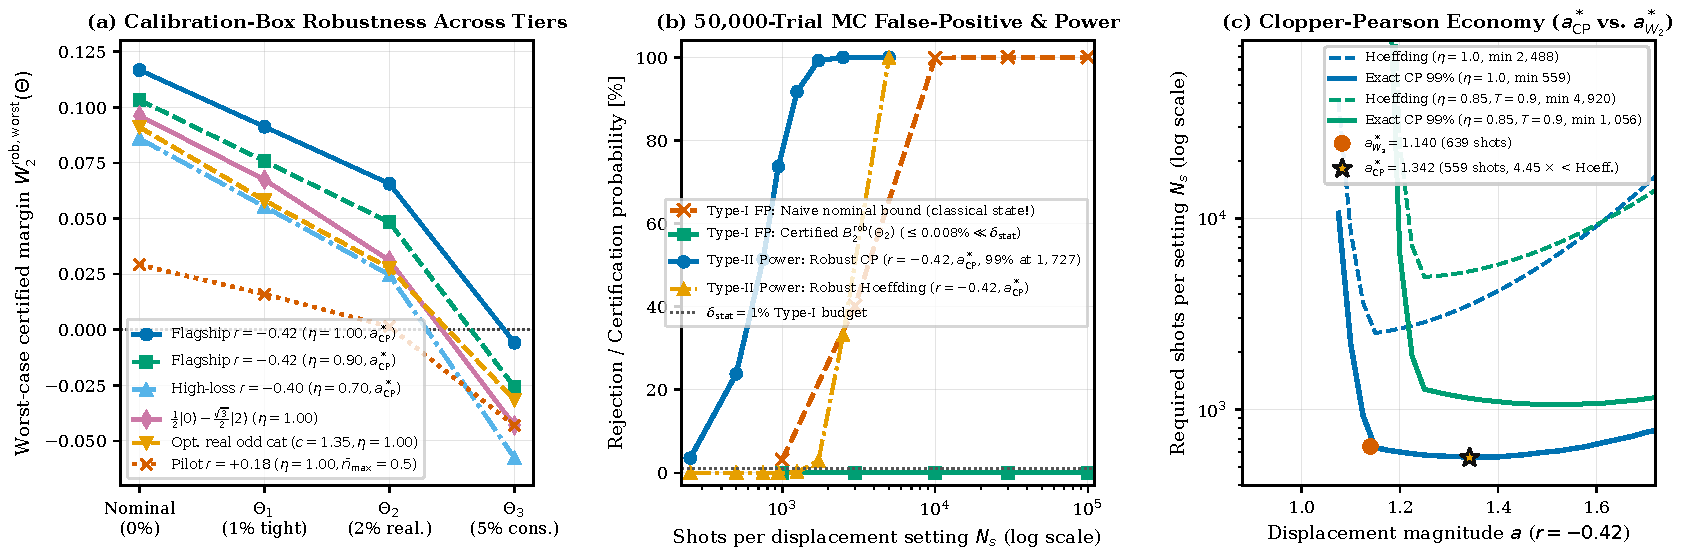
\includegraphics[width=\textwidth]{figures/fig4_calibration_and_stats.pdf}
\caption{\textbf{Asymmetric calibration-box robustness, 50,000-trial Monte Carlo false-positive audit, and Clopper--Pearson shot economy.}
\textbf{(a)}~Worst-case certified margin $W_2^{\rm rob,worst}(\Theta)$ across calibration uncertainty tiers: Nominal ($0\%$), $\Theta_1$ ($1\%$), $\Theta_2$ ($2\%$), and $\Theta_3$ ($5\%$). Flagship $r=-0.42$ ($\eta \in [0.90,1.00]$) and high-loss $r=-0.40$ ($\eta=0.70$) remain robustly positive throughout $\Theta_2$, whereas the $r=+0.18$ pilot collapses to $+0.0014$.
\textbf{(b)}~50,000-trial Monte Carlo audit under $\Theta_2$: testing a classical boundary state against naive nominal $S_2^{\Cset}(\theta_{\rm nom})$ yields up to $100\%$ spurious false positives, whereas certified $B_2^{\rm robust}(\Theta_2)$ holds classical rejection $\le 0.008\% \ll \delta_{\rm stat} = 1\%$ while reaching $99\%$ exact quantum certification power at $1,727$ shots/setting ($r=-0.42, a^*_{\rm CP}=1.342, \eta=1.0$).
\textbf{(c)}~Required shots per setting $N_s(a)$ showing the $4.45\times$ exact Clopper--Pearson speedup over Hoeffding and the calibration headroom gained by shifting from $a^*_{W_2}$ to $a^*_{\rm CP}$.}
\label{fig:fig4}
\end{figure}

Table~\ref{tab:cal-tiers} audits all benchmarks across three asymmetric calibration boxes: $\Theta_1$ (tight: $\abs{\delta a}/a \le 1\%$, $\abs{\delta\eta}\le 0.005$, $\delta\nu \le 10^{-4}$, $\delta_{\phi,\max}=1^\circ$, $+5\%$ cap), $\Theta_2$ (realistic: $2\%, 0.01, 10^{-3}, 2^\circ, +10\%$ cap), and $\Theta_3$ (conservative: $5\%, 0.02, 5\times 10^{-3}, 5^\circ, +20\%$ cap). Crucially, shifting from $a^*_{W_2}$ to the statistical optimum $a^*_{\rm CP}$ provides a \emph{second, independent} advantage: moving to the gentler high-$a$ shoulder of the witness peak cuts calibration-box inflation $\Delta_{\rm cal}(\Theta_2) = B_2^{\rm robust} - S_2^{\Cset}(\theta_{\rm nom})$ (e.g.\ from $0.0394$ to $0.0298$ at $\eta=1.0$), reducing $\Theta_2$ worst-case shots by $2.46\times$ at $\eta=0.90$ ($7,448 \to 3,033$) and $6.92\times$ at $\eta=0.70$ ($91,402 \to 13,201$); re-optimizing the displacement directly against the $\Theta_2$ box ($a^*_{\rm robust,CP}$) lowers these budgets further to $1,630$ ($a=1.482, \eta=1.0$), $2,831$ ($a=1.577, \eta=0.9$), and $11,327$ ($a=1.767, \eta=0.7$). Table~\ref{tab:mc-audit} confirms via 50,000-trial Monte Carlo runs that naive nominal bounds cause $99.8\%$--$100\%$ spurious false positives at $N_s \ge 10{,}000$, while $B_2^{\rm robust}(\Theta_2)$ enforces Type-I control $\le 8 \times 10^{-5}$, and Table~\ref{tab:kov2026-comp} contrasts our protocol explicitly with Kovtoniuk \emph{et al.}~\cite{Kovtoniuk2026}.

\begin{table}[t]
\centering
\caption{\textbf{Globally certified calibration-box audit across Nominal, $\Theta_1$ ($1\%$), $\Theta_2$ ($2\%$), and $\Theta_3$ ($5\%$).} Reports $W_2^{\rm rob}(\theta_{\rm nom}) / W_2^{\rm rob,worst}(\Theta)$ and worst-case shots ($N_s^{\rm CP99,worst}$ at $\delta_{\rm stat}=0.01$, $\delta_{\rm tot} = 0.02$ with $\delta_{\rm cal}=\delta_E=0.005$).}
\label{tab:cal-tiers}
\footnotesize
\setlength{\tabcolsep}{3pt}
\resizebox{\textwidth}{!}{%
\begin{tabular}{@{}lccccc@{}}
\toprule
Benchmark State & $a$ & Nominal $W_2$ ($N_s$) & $\Theta_1$ ($1\%$) & $\Theta_2$ ($2\%$) & $\Theta_3$ ($5\%$) \\
\midrule
Flagship $r=-0.42$ ($\eta=1.0$) & $1.150$ & $+0.1383$ ($630$) & $+0.1185 / +0.1038$ ($1,106$) & $+0.0989 / +0.0690$ ($2,473$) & $+0.0418 / -0.0330$ \\
Flagship $r=-0.42$ ($\eta=1.0$) & $1.342$ & $+0.1168$ ($559$) & $+0.1017 / +0.0913$ (\textbf{904}) & $+0.0870 / +0.0657$ (\textbf{1,727})$^a$ & $+0.0487 / -0.0058$ \\
Flagship $r=-0.42$ ($\eta=0.9$) & $1.191$ & $+0.1272$ ($798$) & $+0.0997 / +0.0839$ ($1,802$) & $+0.0731 / +0.0409$ ($7,448$) & $+0.0110 / -0.0689$ \\
Flagship $r=-0.42$ ($\eta=0.9$) & $1.446$ & $+0.1033$ ($688$) & $+0.0863 / +0.0758$ (\textbf{1,259}) & $+0.0698 / +0.0483$ (\textbf{3,033})$^b$ & $+0.0293 / -0.0258$ \\
High-loss $r=-0.40$ ($\eta=0.7$) & $1.308$ & $+0.1048$ ($1,334$) & $+0.0769 / +0.0585$ ($4,228$) & $+0.0498 / +0.0125$ ($91,402$) & $-0.0142 / -0.1050$ \\
High-loss $r=-0.40$ ($\eta=0.7$) & $1.629$ & $+0.0859$ ($1,123$) & $+0.0681 / +0.0553$ (\textbf{2,669}) & $+0.0507 / +0.0246$ (\textbf{13,201})$^c$ & $+0.0079 / -0.0577$ \\
Pilot $r=+0.18$ ($\nbar=0.50$) & $0.434$ & $+0.0292$ ($12,934$) & $+0.0214 / +0.0160$ ($42,912$) & $+0.0136 / +0.0014$ ($>2\times 10^6$) & $-0.0078 / -0.0431$ \\
Fock $\ket{1}$ ($\eta=1.0$) & $0.433$ & $+0.0311$ ($11,334$) & $+0.0233 / +0.0129$ ($65,950$) & $+0.0156 / -0.0052$ (---) & $-0.0058 / -0.0518$ \\
Opt.\ real odd cat ($c=1.35$) & $0.354$ & $+0.0911$ ($851$) & $+0.0661 / +0.0582$ ($1,985$) & $+0.0435 / +0.0276$ ($8,361$)$^*$ & $+0.0028 / -0.0316$ \\
$\frac{1}{2}\ket{0}-\frac{\sqrt{3}}{2}\ket{2}$ ($\eta=1.0$) & $0.699$ & $+0.0638$ ($789$) & $+0.0598 / +0.0501$ ($1,331$) & $+0.0558 / +0.0361$ ($2,625$)$^{**}$ & $+0.0444 / -0.0008$ \\
\bottomrule
\end{tabular}}
\par\vspace{2pt}\footnotesize\raggedright
At $\Theta_2$-optimized displacements $a^*_{\rm robust,CP}$, worst-case shots drop further to $^a$\textbf{1,630} ($a=1.482$), $^b$\textbf{2,831} ($a=1.577$), $^c$\textbf{11,327} ($a=1.767$), $^*$\textbf{3,003} ($a=0.293$), and $^{**}$\textbf{1,896} ($a=0.816$).
\end{table}

\begin{table}[t]
\centering
\caption{\textbf{50,000-trial Monte Carlo Type-I false-positive audit under $\Theta_2$ ($\delta_{\rm stat}=0.01$)} for the boundary classical mixture $(\theta^*,\mu^*) \in \Theta_2 \times \Cset_{\nU}$ at nominal $a=1.15, \eta=1.0, \nbar=0.22$.}
\label{tab:mc-audit}
\footnotesize
\setlength{\tabcolsep}{3.5pt}
\begin{tabular}{@{}rccccc@{}}
\toprule
$N_s$ & Naive Hoeff. & Naive CP & \textbf{Certified Rob.\ Hoeff.} & \textbf{Certified Rob.\ CP} & Exact PMF Rob.\ CP \\
\midrule
1,000 & 0.00002 & 0.03118 (3.1\%) & \textbf{0.00000} & \textbf{0.00002} ($\le 0.01$) & 0.000027 \\
3,000 & 0.00896 & 0.40208 (40.2\%) & \textbf{0.00000} & \textbf{0.00008} ($\le 0.01$) & 0.000030 \\
10,000 & 0.80488 & 0.99812 (99.8\%) & \textbf{0.00000} & \textbf{0.00002} ($\le 0.01$) & 0.000033 \\
30,000 & 1.00000 & 1.00000 (100\%) & \textbf{0.00000} & \textbf{0.00002} ($\le 0.01$) & 0.000034 \\
100,000 & 1.00000 & 1.00000 (100\%) & \textbf{0.00000} & \textbf{0.00004} ($\le 0.01$) & 0.000035 \\
\bottomrule
\end{tabular}
\end{table}

\begin{table}[t]
\centering
\caption{\textbf{Explicit positioning vs.\ Kovtoniuk--Bohmann--Semenov, Phys.\ Rev.\ A 113, 063726 (2026)~\cite{Kovtoniuk2026}.}}
\label{tab:kov2026-comp}
\small
\begin{tabular}{@{}p{0.21\textwidth}p{0.35\textwidth}p{0.38\textwidth}@{}}
\toprule
Feature & Kovtoniuk \emph{et al.} (PRA 2026)~\cite{Kovtoniuk2026} & Present Work \\
\midrule
Measurement model & Variable-transmittance attenuation channel (no LO displacement). & Two-setting displaced on/off detection with $(a_+,a_-,\delta_\phi,\eta_+,\eta_-,\nu_+,\nu_-)$. \\
Energy information & Unconstrained classical convex hull. & Energy-constrained $\Cset_{\nU}$ + no-go theorem (Prop.~\ref{prop:no-go}) + tap-beam $\nU$ protocol. \\
Calibration robustness & Worst-case classical bound over transmittance calibration intervals. & Global $B_2^{\rm robust}(\Theta,\nU)$ via exact corner reductions + decoupled $C^2$ dual + branch-and-bound ($U-L \le 10^{-8}$). \\
Finite-sample statistics & Asymptotic Gaussian $1\sigma$ error bars on linear inequalities. & Distribution-free exact Clopper--Pearson / Hoeffding LCBs + $\delta_{\rm tot} = \delta_{\rm stat}+\delta_{\rm cal}+\delta_E$ for nonlinear Lorenz sums. \\
\bottomrule
\end{tabular}
\end{table}

% ===========================================================================
\section{Certified Ideal Quantum Ceilings and Finite-Fock Truncation Audit}\label{sec:quantum-ceilings}
% ===========================================================================

To complete the comparison between classical and quantum majorization envelopes without introducing uncertified Fock-space cutoffs, we derive exact ideal quantum ceilings in infinite dimension alongside a quantitative Fock-truncation tail audit.

\begin{proposition}[Exact Zero-Truncation Ideal Quantum Ceilings]\label{prop:quantum-ceilings}
At ideal detection ($\eta = 1, \nu = 0$), let $V_a = \operatorname{span}\{\ket{a}, \ket{-a}\}$ with overlap $g := \braket{-a}{a} = \ee^{-2a^2}$ and orthonormal even/odd cat basis $\ket{\Cset_\pm(a)} = (\ket{a} \pm \ket{-a})/\sqrt{2(1 \pm g)}$. Then on the full infinite-dimensional Hilbert space:
\begin{enumerate}[leftmargin=*]
\item {\normalfont\textbf{\texttt{off/off}}} \textbf{($A_{00} = \ket{-a}\!\bra{-a} + \ket{a}\!\bra{a}$):} $\lambda_{\max}(A_{00}) = 1 + \ee^{-2a^2}$, uniquely attained by the even cat state $\ket{\Cset_+(a)}$ with finite mean photon number $\langle\hat n\rangle = a^2\tanh(a^2)$ (e.g.\ $0.037020$ at $a=0.44$, where the $r=+0.18$ pilot reaches $99.97\%$ of this ceiling).
\item {\normalfont\textbf{\texttt{off/on}}} \textbf{($A_{01} = \I - \ket{-a}\!\bra{-a} + \ket{a}\!\bra{a}$):} Restricting $A_{01} - \I = \sqrt{1-g^2}\,\sigma_x$ in $\{\ket{\Cset_+(a)}, \ket{\Cset_-(a)}\}$ gives $\lambda_{\max}(A_{01}) = 1 + \sqrt{1 - \ee^{-4a^2}}$ ($1.734180$ at $a=0.44$), uniquely attained by $\ket{\psi_{01}^*} = \frac{1}{\sqrt{2}}\bigl(\ket{\Cset_+(a)} + \ket{\Cset_-(a)}\bigr)$ with exact mean photon number $\langle\hat n\rangle = a^2\coth(2a^2)$ ($0.524741$ at $a=0.44$).
\item {\normalfont\textbf{\texttt{on/on}}} \textbf{($A_{11} = 2\I - \ket{-a}\!\bra{-a} - \ket{a}\!\bra{a}$):} $\lambda_{\max}(A_{11}) = 2$, attained on $V_a^\perp$ by the 3-level dark state $\ket{\chi_a}$ of Eq.~\eqref{eq:darkstate} with energy $4/(a^4+2)$ (simultaneously attaining $L_1=1$ and $L_2=2$).
\end{enumerate}
\end{proposition}
\begin{proof}
Because $E_0(\pm a) = \ket{\mp a}\!\bra{\mp a}$ are rank-one projectors, $A_{00}, A_{01}-\I, A_{11}-2\I$ vanish identically on $V_a^\perp$, and diagonalize directly on $V_a$ using $\ket{a}\!\bra{a} + \ket{-a}\!\bra{-a} = (1+g)\ket{\Cset_+}\!\bra{\Cset_+} + (1-g)\ket{\Cset_-}\!\bra{\Cset_-}$ and $\ket{a}\!\bra{a} - \ket{-a}\!\bra{-a} = \sqrt{1-g^2}\bigl(\ket{\Cset_+}\!\bra{\Cset_-} + \ket{\Cset_-}\!\bra{\Cset_+}\bigr)$. Parity invariance $\bra{\Cset_+(a)}\hat n\ket{\Cset_-(a)} = 0$ yields $\bra{\psi_{01}^*}\hat n\ket{\psi_{01}^*} = \frac{a^2}{2}[\tanh(a^2) + \coth(a^2)] = a^2\coth(2a^2)$.
\end{proof}

For general $\eta < 1$ or $\nbar < 4/(a^4+2)$, one can project onto the finite Fock subspace $\mathcal{H}_N = \operatorname{span}\{\ket{0},\dots,\ket{N}\}$ with projector $P_N$ and solve the exact finite-dimensional SDP dual~\eqref{eq:state-sets} for the compressed operator $P_N A P_N$:
\begin{align}\label{eq:fock-sdp-tail}
h_{\Qset_{\nbar}}(A) &\le h_{\Qset_{\nbar}, N}(P_N A P_N) + R_N(m), \\
R_N(m) &:= m\min\bigl\{1,\ \sqrt{\delta_N} + \delta_N/2\bigr\}, \qquad
\delta_N := \min\Bigl(1, \frac{\nbar}{N+1}\Bigr), \nonumber
\end{align}
where the remainder $R_N(m)$ ($0 \preceq A \preceq m\I$) follows from Winter's gentle-projection trace-norm lemma~\cite{Winter1999} applied to $\sigma = P_N\rho P_N + \tr[(\I-P_N)\rho]\ket{0}\!\bra{0}$. Table~\ref{tab:fock-tail} and Figure~\ref{fig:fig5} show that although the compressed Fock SDP stabilizes by $N = 15$ ($1.792833$, SDP gap $\le 2.2\times 10^{-15}$), the generic $O(N^{-1/2})$ tail penalty $R_N(2)$ remains $+0.0673$ even at $N = 200$. Consequently, keeping our witness thresholds exact in the classical sector (zero Fock cutoff) while reporting zero-truncation ideal quantum ceilings (Proposition~\ref{prop:quantum-ceilings}) leaves our nonclassicality certificates completely free of Fock-truncation artifacts.

\begin{figure}[t]
\centering
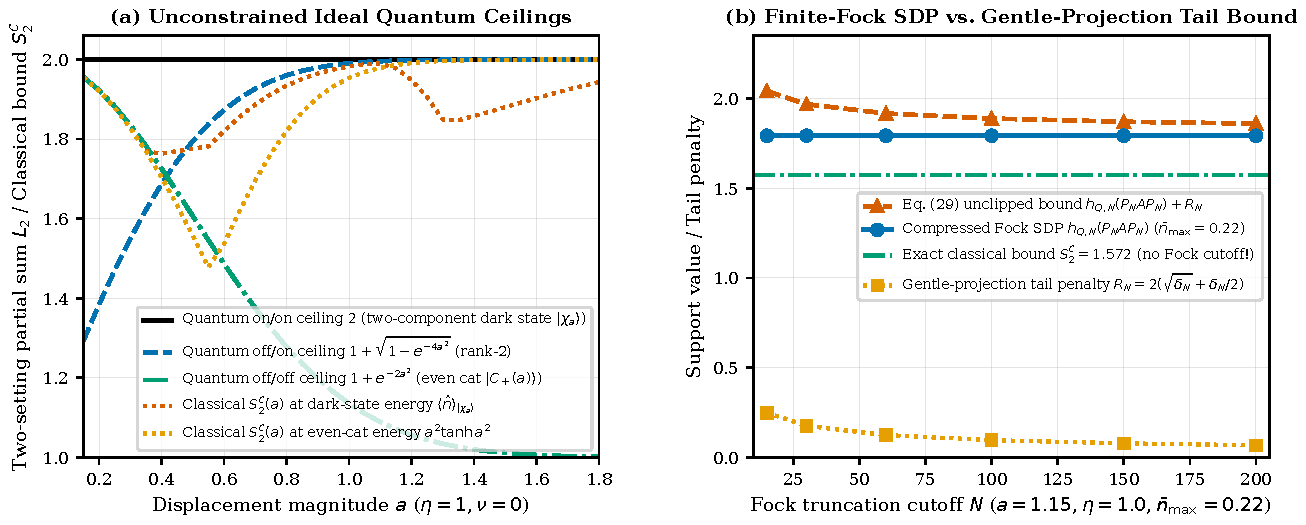
\includegraphics[width=0.92\textwidth]{figures/fig5_quantum_ceilings_audit.pdf}
\caption{\textbf{Exact zero-truncation ideal quantum ceilings and finite-Fock SDP tail audit.}
\textbf{(a)}~Ideal ($\eta=1, \nu=0$) quantum ceilings of Proposition~\ref{prop:quantum-ceilings} (\texttt{on/on} $=2$ by 3-level dark state $\ket{\chi_a}$, \texttt{off/on} $=1+\sqrt{1-\ee^{-4a^2}}$, \texttt{off/off} $=1+\ee^{-2a^2}$ by even cat $\ket{\Cset_+(a)}$) compared against exact classical bounds $S_2^{\Cset}(a)$ at matching state energies.
\textbf{(b)}~At flagship $a = 1.15, \eta = 1.0, \nbar = 0.22$, the compressed Fock SDP $h_{\Qset,N}(P_N A P_N)$ converges by $N = 15$ ($1.792833$, gap $\le 2.2\times 10^{-15}$), while the gentle-projection tail remainder $R_N(2) = 2(\sqrt{\delta_N} + \delta_N/2)$~\cite{Winter1999} decays as $O(N^{-1/2})$ and remains $+0.0673$ at $N = 200$.}
\label{fig:fig5}
\end{figure}

\begin{table}[t]
\centering
\caption{\textbf{Finite-Fock compressed SDP dual vs.\ gentle-projection tail bound~\eqref{eq:fock-sdp-tail}} at $a=1.15, \eta=1.0, \nbar=0.22$ ($S_2^{\Cset} = 1.572308$, zero cutoff).}
\label{tab:fock-tail}
\small
\begin{tabular}{@{}rccccc@{}}
\toprule
$N$ & $h_{\Qset,N}(P_N A P_N)$ & Primal--Dual Gap & $\delta_N = \nbar/(N+1)$ & Remainder $R_N(2)$ & Bound~\eqref{eq:fock-sdp-tail} \\
\midrule
15 & 1.792833 & $2.22 \times 10^{-15}$ & 0.013750 & $+0.248271$ & 2.041104 \\
30 & 1.792833 & $1.11 \times 10^{-15}$ & 0.007097 & $+0.175581$ & 1.968415 \\
60 & 1.792833 & $8.88 \times 10^{-16}$ & 0.003607 & $+0.123716$ & 1.916549 \\
100 & 1.792833 & $1.33 \times 10^{-15}$ & 0.002178 & $+0.095521$ & 1.888354 \\
150 & 1.792833 & $1.55 \times 10^{-15}$ & 0.001457 & $+0.077797$ & 1.870630 \\
200 & 1.792833 & $2.22 \times 10^{-15}$ & 0.001095 & $+0.067262$ & 1.860095 \\
\bottomrule
\end{tabular}
\end{table}

% ===========================================================================
\section{Discussion and Outlook}\label{sec:discussion}
% ===========================================================================

By pairing an independently certified pre-displacement energy constraint $\tr(\rho\hat n) \le \nU$ with two opposite displaced threshold-detector settings, we have resolved the infinite-dimensional $c = 1$ obstruction of binary direct-sum majorization without altering the binary on/off detection hardware. The resulting classical majorization envelope (Theorem~\ref{thm:universal-closed-form}) is exact in closed form across all displacements $a > 0$, detector efficiencies $\eta \in (0,1]$, and dark-count rates $\nu \ge 0$, bounds all Shannon, Tsallis, and R\'enyi entropy sums simultaneously (Lemma~\ref{lem:restricted-binary}), suffers zero sorting penalty on the active click branch (Theorem~\ref{thm:outcome-resolved}), and generalizes cleanly to 7-parameter asymmetric calibration boxes (Theorems~\ref{thm:asym-circle}--\ref{thm:robust-box}) and distribution-free Clopper--Pearson error budgets (Theorem~\ref{thm:finite-sample}).

We emphasize three deliberate scope boundaries and open directions. First, our witness is strictly a \emph{sufficient} nonclassicality certificate: nonviolation of $W_2 > 0$ never implies classicality, and for asymmetric click settings ($q_+ \neq q_-$) full convex-hull membership in $\Dset_{\nbar}$ can outperform sorted majorization. Second, tighter operator-adapted spectral tail bounds beyond generic trace-norm gentle projection~\eqref{eq:fock-sdp-tail} remain an interesting mathematical problem for $\eta < 1$ quantum majorization envelopes~\cite{YangQiaoOptimization2026}. Third, our single-mode, two-setting protocol opens natural extensions to continuous-variable steering, multimode entangled threshold networks, and experimental demonstrations using standard $\approx 3.5\;\mathrm{dB}$ squeezed vacuum sources and tap-beam power monitors.

\section*{Data and Code Availability}
All analytical solvers, $C^2$-certified dual routines, Fock-space Kraus-channel tests (51 unit tests passing), CSV datasets, and plotting scripts reproducing every number, table, and figure in this manuscript are publicly available at \url{https://github.com/RuiZhu1/quantum-light-majorization} and can be executed end-to-end via \texttt{python run\_all.py}.

\section*{Acknowledgments}
We acknowledge helpful discussions with Gilad Gour on binary direct-sum majorization and support from Guangdong Technion -- Israel Institute of Technology.

% ===========================================================================
\appendix
\section{Technical Proofs}\label{app:proofs}
% ===========================================================================

\subsection{Proof of Theorem~\ref{thm:concavity} (Exact Branch Concavity Thresholds)}\label{app:concavity}
Writing $G(x) = g(x^2)$ ($x = \sqrt{s} > 0$), $g''(s) = \bigl[x G''(x) - G'(x)\bigr]/(4x^3)$, so $\sgn g''(s) = \sgn[x G''(x) - G'(x)]$.
\begin{enumerate}[leftmargin=*]
\item For $g_0(s) = \kappa\ee^{-(x-b)^2}$ on $(0,b)$, $\frac{4x^3}{\kappa\ee^{-(x-b)^2}}g_0''(s) = 2[2x(b-x)^2 - b]$. On $[0,b]$, $2x(b-x)^2$ achieves its unique maximum $\frac{8}{27}b^3$ at $x = b/3$; hence $g_0'' \le 0$ on $(0,b^2]$ iff $b^2 \le \frac{27}{8}$.
\item For $g_{01}(s)$ on $(0, x_*]$, $\frac{4x^3}{\kappa\ee^{-(x-b)^2}}g_{01}''(s) = 2\bigl[(2x(x-b)^2 - b) - (2x(x+b)^2 + b)\ee^{-4bx}\bigr]$. On $(b, x_*]$, $g_{01}' \ge 0$ implies $(x+b)\ee^{-4bx} \ge x-b > 0$; substituting this yields $[2x(x-b)^2-b] - (2x(x+b)^2+b)\ee^{-4bx} \le -4bx(x-b) - b(1+\ee^{-4bx}) < 0$ for all $b > 0$. On $(0,b]$, the subtracted term is $>0$, so $b^2 \le 27/8$ guarantees $g_{01}'' < 0$ strictly (extending numerically up to $b_{\rm crit,01} \approx 1.874331$).
\item For $g_{00}(s)$ when $2b^2 > 1$, set $z := 2bx > 0$ and $u := 1/b^2 \in (0,2)$:
\begin{equation}\label{eq:Qz-def}
\frac{4x^3 \ee^{x^2+b^2}}{\kappa\cosh z}\,g_{00}''(s) = z^3\left[u^2 - \frac{4\tanh z}{z}\,u + \frac{4(z-\tanh z)}{z^3}\right] =: z^3 Q_z(u).
\end{equation}
As $z \to 0^+$, $Q_0(u) = u^2 - 4u + \frac{4}{3}$ vanishes at $u_1 := 2 - \frac{2\sqrt{6}}{3} = \frac{2}{3+\sqrt{6}}$ ($b_{\rm crit,00}^2 = \frac{3+\sqrt{6}}{2}$). For $u < u_1$, $g_{00}''(0^+) > 0$. Conversely, for $u \in [u_1, 2)$, on $(0, x_0]$ we have $u \le \frac{2\tanh z}{z} = u_{\rm vertex}(Q_z)$, so $Q_z(u) \le Q_z(u_1)$, while $z = 2bx \le 2b^2\tanh z < \frac{2}{u_1} = 3 + \sqrt{6} \approx 5.4495$. Expanding $\sinh z$ and $\cosh z$ in Taylor series yields the positive series
\begin{equation}\label{eq:sinh-pade}
\sinh z\,(105 + 45z^2 + z^4) - z\cosh z\,(105 + 10z^2) = \sum_{k=4}^\infty \frac{16k(k-1)(k-2)(k-3)}{(2k+1)!}\,z^{2k+1} > 0 \quad (\forall z > 0),
\end{equation}
whence $\tanh z > \frac{z(105+10z^2)}{105+45z^2+z^4}$. Using $u_1^2 = 4u_1 - \frac{4}{3}$, direct algebra gives $(105+10z^2)(1+u_1 z^2) - (105+45z^2+z^4)(1+\frac{u_1^2}{4}z^2) = (14 - 35u_1)z^4 - \frac{u_1^2}{4}z^6 > 0$ for all $0 < z < \sqrt{4(14-35u_1)/u_1^2} \approx 5.856$ (covering $(0, 3+\sqrt{6}]$), proving $\tanh z > \frac{z+(u_1^2/4)z^3}{1+u_1 z^2} \iff Q_z(u_1) < 0$. \qedhere
\end{enumerate}

\subsection{Proof of Theorem~\ref{thm:universal-closed-form} (Global Click-Branch Dominance)}\label{app:universal}
We verify strict dominance on every bitangent interval $[s_L, s_R]$ where Theorem~\ref{thm:concavity} permits two-point mixtures:
\begin{enumerate}[leftmargin=*]
\item For $A_{00}$ ($b^2 > \frac{3+\sqrt{6}}{2}$): for every $E \ge 0$, $h_{00}(E) \le \kappa(1+\ee^{-b^2})$ while $h_{11}(E) \ge 2 - 2\kappa\ee^{-b^2}$, so $h_{11}(E) - h_{00}(E) \ge 2 - \kappa(1 + 3\ee^{-b^2}) \ge 1 - 3\ee^{-(3+\sqrt{6})/2} > 0.80 > 0$.
\item For $E_0$ ($b^2 > \frac{27}{8}$): on $[s_L, s_R] \subset (0, b^2)$, $h_0(E) \le g_0(s_R)$. The tangent intercept $I_0(s) := g_0(s) - s g_0'(s)$ increases on $(x_2^2, b^2)$ ($I_0' = -s g_0'' > 0$) and satisfies $I_0(s_R) = I_0(s_L) < g_0(s_L) < \kappa\ee^{-4b^2/9} < 0.224\kappa$ (since $x_1 < b/3$). Evaluating at $x = b - \frac{1}{2b} \in (x_2, b)$ gives $I_0(x^2) = \kappa\ee^{-1/(4b^2)}(\frac{1}{2} + \frac{1}{4b^2}) > 0.464\kappa > 0.224\kappa$, forcing $b - x_R > \frac{1}{2b}$. Hence $h_1(E) - h_0(E) > 1 - \kappa(\ee^{-b^2} + \ee^{-1/(4b^2)}) \ge 1 - (\ee^{-t} + \ee^{-1/(4t)}) > 0$ for all $t = b^2 \ge \frac{27}{8}$ (using $\ee^{-1/(4t)} < 1 - \frac{7}{32t}$ and $t\ee^{-t} < \frac{7}{32}$).
\item For $A_{01}$ ($b \ge b_{\rm crit,01} \approx 1.8743$, $b^2 \ge 3.5131$): let $\tilde g_{01}(s) := g_{01}(s) - 1$. Its inflection point satisfies $x_1^{01} < b/2$, so $\tilde I_{01}(s_R) = \tilde I_{01}(s_L) < \tilde g_{01}(s_L) < \kappa\ee^{-b^2/4} \le 0.4155\kappa < 0.50\kappa < \tilde I_{01}((b - \frac{1}{2b})^2)$, again forcing $b - x_R > \frac{1}{2b}$. Then $h_{11}(E) - h_{01}(E) > 1 - (2\ee^{-t} + \ee^{-1/(4t)}) > 0$ since $2t\ee^{-t} \le 0.2093 < \frac{7}{32}$ for all $t \ge 3.5131$. \qedhere
\end{enumerate}

\subsection{Proofs of Theorems~\ref{thm:asym-circle} and~\ref{thm:robust-box} (Asymmetric Duality and Boxes)}\label{app:calibration}
At fixed $s > 0$ and $\delta_\phi = 0$, differentiating $f_{01}(\varphi) = 1 + C_- \ee^{B_- z} - C_+ \ee^{-B_+ z}$ in $z = \cos\varphi \in [-1,1]$ yields $\partial_z f_{01} = B_- C_- \ee^{B_- z} + B_+ C_+ \ee^{-B_+ z} > 0$, giving $z^* = +1$ (and $z^* = -1$ for $f_{10}$). For $f_{00}$, $\partial_z^2 f_{00} = B_+^2 C_+ \ee^{-B_+ z} + B_-^2 C_- \ee^{B_- z} > 0$, whereas $\partial_z^2 f_{11} = -\partial_z^2 f_{00} < 0$, yielding $z^* \in \{-1,+1\}$ for \texttt{off/off} and $\partial_z f_{11} = 0 \implies z^*(s)$ in Eq.~\eqref{eq:zstar-onon} for \texttt{on/on}. For $\abs{\delta_\phi} \le \delta_{\phi,\max} < \pi/2$, by rotation invariance of the circle, the angular separation between $-\alpha_+$ and $-\alpha_-$ is $\Delta = \pi - \abs{\delta_\phi}$, decreasing with $\abs{\delta_\phi}$; thus \texttt{off/on} contrast peaks at $\delta_\phi = 0$ ($\Delta = \pi$), whereas \texttt{off/off} and \texttt{on/on} peak at $\abs{\delta_\phi} = \delta_{\phi,\max}$ (with bisector $\varphi^* = \delta_\phi/2 - \pi/2$ in the symmetric-magnitude case, giving Eq.~\eqref{eq:onon-dphi}).

In Theorem~\ref{thm:robust-box}, $E_0(j;\theta)$ decreases pointwise in $(a_j,\eta_j,\nu_j)$ at optimal real states while $E_1(j;\theta)$ increases pointwise in $(a_j,\eta_j,\nu_j)$ at $\ket{\pm\sqrt{\nU}}$, reducing $S_1^{\rm robust}$ to exact corner evaluations. Similarly, pointwise monotonicity in $\nu_\pm$ fixes $(\nu_+,\nu_-)$ per cross branch. On any 4D sub-box $B = B_+ \times B_-$, because $\sup_{\theta \in B} \int f_A(\beta;\theta)\,\dd\mu(\beta) \le \int F_A^B(\beta)\,\dd\mu(\beta)$ for every $\mu \in \Cset_{\nU}$, optimizing the single-variable Lagrangian $\lambda \nU + \sup_{\beta}[F_A^B(\beta) - \lambda\abs{\beta}^2]$ over radial shells via $C^2$ second-derivative interval padding certifies $U_A(B) \ge \sup_{\theta\in B} h_{\Cset_{\nU}}(A(\theta))$; adaptive branch-and-bound narrows $U_A - L_A$ to $\le 10^{-8}$. \qedhere

\bibliographystyle{unsrtnat}
\bibliography{references}

\end{document}
